% Options for packages loaded elsewhere
\PassOptionsToPackage{unicode}{hyperref}
\PassOptionsToPackage{hyphens}{url}
\PassOptionsToPackage{dvipsnames,svgnames,x11names}{xcolor}
%
\documentclass[
  12,
  letterpaper,
  DIV=11,
  numbers=noendperiod]{scrartcl}

\usepackage{amsmath,amssymb}
\usepackage{setspace}
\usepackage{iftex}
\ifPDFTeX
  \usepackage[T1]{fontenc}
  \usepackage[utf8]{inputenc}
  \usepackage{textcomp} % provide euro and other symbols
\else % if luatex or xetex
  \usepackage{unicode-math}
  \defaultfontfeatures{Scale=MatchLowercase}
  \defaultfontfeatures[\rmfamily]{Ligatures=TeX,Scale=1}
\fi
\usepackage{lmodern}
\ifPDFTeX\else  
    % xetex/luatex font selection
    \setmainfont[]{Times New Roman}
    \setsansfont[]{Garamond}
  \setmathfont[]{Cambria Math}
\fi
% Use upquote if available, for straight quotes in verbatim environments
\IfFileExists{upquote.sty}{\usepackage{upquote}}{}
\IfFileExists{microtype.sty}{% use microtype if available
  \usepackage[]{microtype}
  \UseMicrotypeSet[protrusion]{basicmath} % disable protrusion for tt fonts
}{}
\makeatletter
\@ifundefined{KOMAClassName}{% if non-KOMA class
  \IfFileExists{parskip.sty}{%
    \usepackage{parskip}
  }{% else
    \setlength{\parindent}{0pt}
    \setlength{\parskip}{6pt plus 2pt minus 1pt}}
}{% if KOMA class
  \KOMAoptions{parskip=half}}
\makeatother
\usepackage{xcolor}
\setlength{\emergencystretch}{3em} % prevent overfull lines
\setcounter{secnumdepth}{-\maxdimen} % remove section numbering
% Make \paragraph and \subparagraph free-standing
\makeatletter
\ifx\paragraph\undefined\else
  \let\oldparagraph\paragraph
  \renewcommand{\paragraph}{
    \@ifstar
      \xxxParagraphStar
      \xxxParagraphNoStar
  }
  \newcommand{\xxxParagraphStar}[1]{\oldparagraph*{#1}\mbox{}}
  \newcommand{\xxxParagraphNoStar}[1]{\oldparagraph{#1}\mbox{}}
\fi
\ifx\subparagraph\undefined\else
  \let\oldsubparagraph\subparagraph
  \renewcommand{\subparagraph}{
    \@ifstar
      \xxxSubParagraphStar
      \xxxSubParagraphNoStar
  }
  \newcommand{\xxxSubParagraphStar}[1]{\oldsubparagraph*{#1}\mbox{}}
  \newcommand{\xxxSubParagraphNoStar}[1]{\oldsubparagraph{#1}\mbox{}}
\fi
\makeatother


\providecommand{\tightlist}{%
  \setlength{\itemsep}{0pt}\setlength{\parskip}{0pt}}\usepackage{longtable,booktabs,array}
\usepackage{calc} % for calculating minipage widths
% Correct order of tables after \paragraph or \subparagraph
\usepackage{etoolbox}
\makeatletter
\patchcmd\longtable{\par}{\if@noskipsec\mbox{}\fi\par}{}{}
\makeatother
% Allow footnotes in longtable head/foot
\IfFileExists{footnotehyper.sty}{\usepackage{footnotehyper}}{\usepackage{footnote}}
\makesavenoteenv{longtable}
\usepackage{graphicx}
\makeatletter
\newsavebox\pandoc@box
\newcommand*\pandocbounded[1]{% scales image to fit in text height/width
  \sbox\pandoc@box{#1}%
  \Gscale@div\@tempa{\textheight}{\dimexpr\ht\pandoc@box+\dp\pandoc@box\relax}%
  \Gscale@div\@tempb{\linewidth}{\wd\pandoc@box}%
  \ifdim\@tempb\p@<\@tempa\p@\let\@tempa\@tempb\fi% select the smaller of both
  \ifdim\@tempa\p@<\p@\scalebox{\@tempa}{\usebox\pandoc@box}%
  \else\usebox{\pandoc@box}%
  \fi%
}
% Set default figure placement to htbp
\def\fps@figure{htbp}
\makeatother
% definitions for citeproc citations
\NewDocumentCommand\citeproctext{}{}
\NewDocumentCommand\citeproc{mm}{%
  \begingroup\def\citeproctext{#2}\cite{#1}\endgroup}
\makeatletter
 % allow citations to break across lines
 \let\@cite@ofmt\@firstofone
 % avoid brackets around text for \cite:
 \def\@biblabel#1{}
 \def\@cite#1#2{{#1\if@tempswa , #2\fi}}
\makeatother
\newlength{\cslhangindent}
\setlength{\cslhangindent}{1.5em}
\newlength{\csllabelwidth}
\setlength{\csllabelwidth}{3em}
\newenvironment{CSLReferences}[2] % #1 hanging-indent, #2 entry-spacing
 {\begin{list}{}{%
  \setlength{\itemindent}{0pt}
  \setlength{\leftmargin}{0pt}
  \setlength{\parsep}{0pt}
  % turn on hanging indent if param 1 is 1
  \ifodd #1
   \setlength{\leftmargin}{\cslhangindent}
   \setlength{\itemindent}{-1\cslhangindent}
  \fi
  % set entry spacing
  \setlength{\itemsep}{#2\baselineskip}}}
 {\end{list}}
\usepackage{calc}
\newcommand{\CSLBlock}[1]{\hfill\break\parbox[t]{\linewidth}{\strut\ignorespaces#1\strut}}
\newcommand{\CSLLeftMargin}[1]{\parbox[t]{\csllabelwidth}{\strut#1\strut}}
\newcommand{\CSLRightInline}[1]{\parbox[t]{\linewidth - \csllabelwidth}{\strut#1\strut}}
\newcommand{\CSLIndent}[1]{\hspace{\cslhangindent}#1}

\usepackage{booktabs}
\usepackage{caption}
\usepackage{longtable}
\usepackage{colortbl}
\usepackage{array}
\usepackage{anyfontsize}
\usepackage{multirow}
\usepackage{sectsty}
\sectionfont{\centering}
\subsectionfont{\raggedright}
\usepackage{indentfirst}
\setlength{\parindent}{3em}
\usepackage{amsmath}
\usepackage{amssymb}
\usepackage{enumitem}
\setlist[itemize]{topsep=0pt,itemsep=0pt,partopsep=0pt,parsep=0pt}
\setlist[enumerate]{topsep=0pt,itemsep=0pt,partopsep=0pt,parsep=0pt}
\usepackage{booktabs}
\KOMAoption{captions}{tablesignature}
\makeatletter
\@ifpackageloaded{caption}{}{\usepackage{caption}}
\AtBeginDocument{%
\ifdefined\contentsname
  \renewcommand*\contentsname{Table of contents}
\else
  \newcommand\contentsname{Table of contents}
\fi
\ifdefined\listfigurename
  \renewcommand*\listfigurename{List of Figures}
\else
  \newcommand\listfigurename{List of Figures}
\fi
\ifdefined\listtablename
  \renewcommand*\listtablename{List of Tables}
\else
  \newcommand\listtablename{List of Tables}
\fi
\ifdefined\figurename
  \renewcommand*\figurename{Figure}
\else
  \newcommand\figurename{Figure}
\fi
\ifdefined\tablename
  \renewcommand*\tablename{Table}
\else
  \newcommand\tablename{Table}
\fi
}
\@ifpackageloaded{float}{}{\usepackage{float}}
\floatstyle{ruled}
\@ifundefined{c@chapter}{\newfloat{codelisting}{h}{lop}}{\newfloat{codelisting}{h}{lop}[chapter]}
\floatname{codelisting}{Listing}
\newcommand*\listoflistings{\listof{codelisting}{List of Listings}}
\makeatother
\makeatletter
\makeatother
\makeatletter
\@ifpackageloaded{caption}{}{\usepackage{caption}}
\@ifpackageloaded{subcaption}{}{\usepackage{subcaption}}
\makeatother

\usepackage{bookmark}

\IfFileExists{xurl.sty}{\usepackage{xurl}}{} % add URL line breaks if available
\urlstyle{same} % disable monospaced font for URLs
\hypersetup{
  pdftitle={Too hard to get: the role of probabilistic expectations and cognitive complexity in multi-dimensional reference dependence},
  pdfauthor={Aspen Han},
  colorlinks=true,
  linkcolor={blue},
  filecolor={Maroon},
  citecolor={Blue},
  urlcolor={Blue},
  pdfcreator={LaTeX via pandoc}}


\title{Too hard to get: the role of probabilistic expectations and
cognitive complexity in multi-dimensional reference dependence}
\author{Aspen Han}
\date{}

\begin{document}
\maketitle
\begin{abstract}
This paper seeks to investigate the effects of conflicting reference
points across different dimensions of utility on effort exertion.
Reference-dependent preference models so far have assumed additive
separability across different dimensions of utility, which implies that
agents respond to reference points in each dimension in isolation from
one another. Challenging this assumption, this paper posits that agents
consider multi-dimensional reference points in tandem: agents are less
responsive to reference points if they have low probabilistic
expectations of being able to concurrently achieve them and/or if they
have difficulty reconciling them into a single baseline against which to
evaluate outcomes. It refines the Koszegi-Rabin reference-dependent
preference model to incorporate these effects and applies it to examine
effort exertion under targets in different task performance dimensions.
The original and refined model produce distinct predictions for optimal
effort exertion, which are tested via a real effort experiment. However,
the experimental results are inconclusive, finding some evidence of
attenuation but which is not statistically significant nor robust. They
do shed light on dynamics between internally conceived and externally
imposed targets and how they enter into reference point formation which
has bearing for target design and can be a promising new area of
research for the future.
\end{abstract}


\setstretch{2}
\section{Introduction}\label{introduction}

Consider the employee of a firm whose performance is evaluated against
targets across various performance dimensions (e.g.~production speed,
accuracy, quality etc). For example, an assembly line worker in an
electronics manufacturing plant could be subject to targets on the
number of components made per hour (speed), the proportion of defective
components made (accuracy), and the average durability of components
made (quality). Similarly in the service sector, an Uber driver could be
evaluated on the number of rides provided per month, average mileage per
unit time, and the average customer satisfaction rating. It is apparent
that tensions between these performance dimensions can surface, which
can affect the targets' effectiveness as motivators. The emphasis for
consistency and complementarity between different performance
dimensions, including targets set in each, is strongly echoed in
operations and general management literature (e.g. Hayes 1984; Hayes and
Schmenner 1978; Skinner 1974, 1996; Swamidass and Darlow 2000). Further
insights can be gleaned from examining this concept within economics.
Targets can and have been integrated into the framework of
expectations-based reference points (Heath, Larrick, and Wu 1999; Von
Rechenberg, Gutt, and Kundisch 2016), a growing body of research within
behavioral economics. However, empirical studies have mainly examined
the effects of reference points uni-dimensionally, though theoretical
models encompassing multi-dimensional reference points exist. Thus, I
seek to investigate the mechanisms through which reference points
interact across dimensions within this economic framework, specifically
answering the following research questions:

\begin{enumerate}
\def\labelenumi{\arabic{enumi}.}
\tightlist
\item
  Do probabilistic beliefs about the achievability of reference points
  across multiple dimensions affect how responsive agents are to said
  reference points?
\item
  Does cognitive complexity in reconciling reference points across
  multiple dimensions affect how responsive agents are to said reference
  points?
\end{enumerate}

This research is theoretically founded on the Koszegi and Rabin (2006)
model of reference-dependence (henceforth KR model), which builds upon
Kahneman and Tversky's (1979; 1991) prospect theory and related models
of regret and disappointment (e.g. Bell 1982, 1985; Loomes and Sugden
1982, 1986; Gul 1991). Defining features of this overarching framework
include the evaluation of outcomes relative to a reference point rather
than on absolute terms, weighting losses more than gains, diminishing
sensitivity away from the reference point, and decision weights on
outcomes which are transformations of objective probabilities. A major
contribution by the KR model is that it constructs a source for the
reference points to be the agent's (rational) expectations, specifically
his/her probabilistic beliefs held in the recent past about what will or
should happen. This accommodated alternative arguments about the origins
of reference points, which had been contended to be the status quo by
some (e.g. Genesove and Mayer 2001; Kahneman, Knetsch, and Thaler 1990)
but also refuted by other (e.g. Plott and Zeiler 2005; Tversky and
Kahneman 1991). Pinpointing the source of reference points allowed for
more detailed studies into their manipulability from a policy
perspective, which motivates my use of the KR model as a theoretical
baseline. The model also generalizes to multiple dimensions of
consumption, increasing portability to the conventional consumer choice
problems in economics. While there remains a continued debate about the
source of reference points, this paper abstracts away from that and
instead focuses on whether the KR model is a good description of
behavior with respect to reference points across multiple dimensions
within the framework of expectations-based reference point. Similar to
other expected utility and reference-dependent models, the KR model
assumes that utilities across different dimensions of consumption are
additively separate, which I seek to challenge. Given the motivating
example highlighted above, it seems unrealistic to think that people
would view reference points in each dimension in isolation from one
another and determine how much to work towards each with complete
disregard for the others.

The interaction effects between reference points across dimensions had
been largely neglected despite a rich empirical literature in the
expectations-based reference points. Crawford and Meng (2011) found that
the work patterns of New York taxi drivers could be explained by the KR
model with dual reference points in daily wages earned and hours worked.
While this is one of few works to consider multi-dimensional reference
points, the field context made it difficult to elucidate the reference
points, much less the mechanisms through which they could have
interacted and affected the drivers' work behavior. Furthermore, since
the taxi drivers are independent contractors, their reference points are
self-imposed and hence likely consistent by construction, whereas
conflicting effects are the focus of my research questions. Abeler et
al. (2011) tested and verified the KR model in a laboratory experiment
where subjects were set reference points in earnings and then asked to
work on a real effort task. The controlled setting allowed the reference
points to be exogenously induced so their effects on effort provision
could be explicated. However, they only considered a reference point in
a single dimension and hence neglected multi-dimensional interaction
effects. Thus, synthesizing the laboratory methodology of Abeler et
al.~and the dual reference point model of Crawford and Meng, my
undergraduate research sought to test the multi-dimensional version of
the KR model. It found that when the two reference points were
congruent, they had reinforcing effects, which fits with KR model
predictions, but when they were conflicting, they had negating effects
in that subjects seemed to ignore the reference points completely
instead of compromising between them or prioritizing one over the other
as predicted by the KR model. This leads to my research questions, which
endeavor to identify the reasons behind this destructive effect between
disparate reference points in different dimensions.

I propose two main explanations: agents are unresponsive to reference
points when they perceive the probability of being able to achieve them
concurrently to be low, and/or when they find it cognitively complex to
reconcile the reference points. These problems arise when reference
points across multiple dimensions conflict. These stem from ideas in the
management literature as discussed above and could link to the successes
of managerial philosophies and practices such as Total Quality
Management which emphasize a holistic consideration of organizational
performance and are able to integrate potentially conflicting
performance dimensions. We can capture these effects by appending to the
KR model additional parameters which scale the gain-loss utility
components, which would alter the first-order conditions predicting
optimal effort provision such that they align with the experimental
results.

I tested these propositions with a laboratory experiment. I elected for
an experimental methodology as I wanted to clearly identify the
decision-making mechanisms which integrate multi-dimensional reference
points, and this is most clearly elicited in the controlled experiments,
being difficult to establish with observational data where the reference
points are elusive and there are many potential confounds. While I have
linked my research motivations to the workplace, the foremost step would
be to uncover the general ways in which people perceive and respond to
multi-dimensional reference points which are applicable to various
contexts, so the abstract setting of the laboratory experiments is
well-suited for it. It also provides a less costly way to verify the
hypothesized mechanisms at work, so it can be thought of as a pilot for
further field research.

In the experiment, subjects worked on a real effort task where they have
to drag sliders along a scale of 0 to 100 to designated numbers. They
were evaluated on speed as measured by the number of slider sets
completed in the alloted time and accuracy as measured by the proportion
of correctly completed sets among sets attempted, with set targets for
each peformance measure. These two performance dimensions have inherent
trade-offs as improving in accuracy necessitates spending more time on
each slider to position it correctly and thus compromising on speed. The
treatments varied the difficulty of achieving the targets, which augment
the probabilistic expectations of simultaneous target achievement, and
the extent of explanation provided regarding the relationship between
the two performance dimensions and their targets, which affect the
cognitive complexity of reconciling them.

However, the experimental findings are inconclusive, mainly because
subjects inherently valued performance in accuracy much more than speed,
with most already achieving beyond the accuracy target in the absence of
it in the control. Thus, the targets introduced externally by the
experimenter have to compete with the internally conceived targets of
the subject, which led to weak and ambiguous reference point effects at
baseline, making it difficult to detect variations of such effects
between treatment groups. There was some evidence of subjects focusing
more on speed at the expense of accuracy upon imposing the external
targets, and of a smaller shift only in the treatment where the targets
were more difficult to achieve simultaneously, though the statistical
support is quite weak. The experimental parameters could have been
better calibrated to strengthen its construct validity for testing
between the original and augmented reference-dependent preference
models. Proper pilots would have been very beneficial for this purpose,
but due to time and budgetary constraints, were not possible.

Nevertheless, the experiment demonstrates another interesting result:
the conflict between internal and external reference points which could
be a major source of friction in workplace motivation. This highlights a
potential exciting area of research with implications for contract
design; specifically employers need to be mindful of employees' internal
values and goals in setting work objectives and incentives for them.
Investigating deeper into the dynamics of how we compromise between
these two expectation-forming environments could reveal new solutions to
contract design.

\section{Design}\label{design}

\subsection{Experimental design}\label{experimental-design}

The experiment is divided into two parts: a real effort task and then a
questionnaire. The former provides the main data on task performance and
effort exertion to answer the research questions, whereas the latter
provides covariate data to improve the precision of estimates and
conduct heterogeneity analysis. There are aspects of the actual
experiment conducted which depart from the ideal design due to resource
constraints and they could have contributed to the inconclusive
findings. I also address these flaws in the design outline below,
including a discussion of the trade-offs, implications, and remedies.

The real effort task is a slider task which consists of a series of
slider sets, and each set contains three sliders which can be moved
along a scale of 0 to 100 (Figure~\ref{fig-slider-set-example}).
Subjects were given five minutes to work on the task. Proceeding to the
next set counts as an attempt of the current set. To complete a set,
subjects had to drag all sliders to within plus or minus ten of their
respective designated numbers on the scale\footnote{There was still some
  element of accuracy in the speed requirement intended to better
  parallel real life work where job completion generally requires some
  minimum quality standard, and to make it more stimulating/ rewarding
  compared to mindless dragging to prevent subjects from gravitating
  towards the accuracy dimension.}. To \emph{correctly} complete a set,
subjects needed to drag every slider to its designated number exactly,
otherwise the set would be counted as mistake. These separate metrics
induce effort in the speed and accuracy dimensions which are in tension
with each other, as performing better on accuracy requires the subject
to spend more time precisely positioning each slider rather than
completing more sets which leads to worse performance on speed. After
being introduced to the task, subjects had 1 minute to work on a demo
task to familiarise themselves with it before receiving further
instructions (related to their treatment group) and working on the
actual task.

In the task, each set was displayed on a separate page, so having
multiple sliders in each set increases the proportion of time actually
spent working on the slider task by reducing the time spent on page
transitions, but too many would have reduced the sensitivity of the
effort measure: tasks (correctly) completed, to effort exerted, so I
decided on three. On every page during the task, subjects were shown key
task performance metrics, including their time spent working up till the
current set, total number of sets attempted, total number of sets
completed, and total actual mistakes made. Scoring was at the set level
instead of the slider level so that the metrics had smaller quantities
and could be more easily processed by subjects while they worked on the
task.

\begin{figure}

\centering{

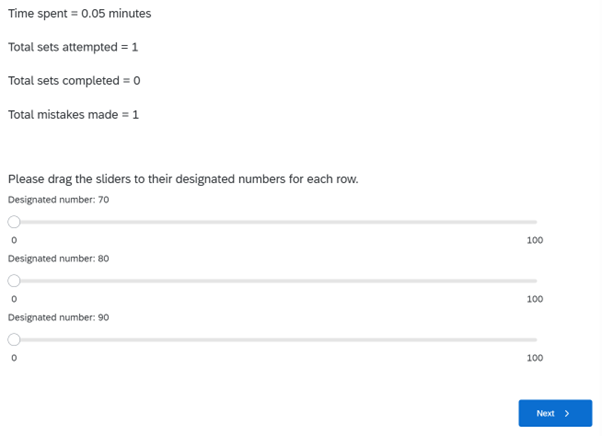
\includegraphics[width=0.75\linewidth,height=\textheight,keepaspectratio]{survey-screenshots/slider-task-set-example.png}

}

\caption{\label{fig-slider-set-example}Example of a set in the slider
task}

\end{figure}%

The slider task was selected because it is mundane and repetitive, hence
reasonably incurring a positive effort cost. This combined with the fact
that working on the task provides no intrinsic value should make it
inert to variation in personal motivation regarding the task. The task
is also easy and intuitive so task performance will be less affected by
differences in intelligence and education/ training among subjects, and
more clearly maps from effort exertion. These will help to reduce noise
in the effort measures. The task is also intentionally abstract in
nature and generic in its assessment since this study seeks to find
universal decision-making processes regarding effort exertion under
reference point effects which has generalisability to a broad range of
jobs and possibly even beyond the labour supply domain. The short task
duration and low stakes may be unrealistic compared to long-term jobs,
but have to be imposed for practical reasons, and still offers insight
into how people respond to multi-dimensional targets at the task level
of a job (e.g.~a single ride for an Uber driver), which can plausibly be
aggregated to the job level. Overall, the objective is not to exactly
capture how people work under targets in specific jobs, but identify
fundamental decision-making mechanisms which can apply to various
domains and vary across them as permitted by the parameters in the
model.

There were four treatment groups which varied the task parameters in
terms of the reference points (i.e.~targets) and how the work was
assessed. Reference points were set in the two performance dimensions:
speed as measured by the number of sets completed, and accuracy as
measured by the proportion of \emph{recorded} mistakes out of sets
attempted. Work was assessed by either of two criteria: strict which
records all actual mistakes made, and lenient which records only a
quarter. The probability for each criterion differs across treatments.
Subjects who are more likely to be assessed by a strict criterion thus
have a lower likelihood of achieving both reference points concurrently.
To reinforce this perception, subjects were primed to think that
``achieving both targets {[}was{]} manageable under a lenient criterion
but highly challenging under a strict criterion''. Reference points were
also either presented as is or explained in greater detail by
explicating how performance in the speed dimension relates to that in
the accuracy dimension. The explanation constituted a table showing the
maximum number of total actual mistakes allowed under each criterion for
different number of total tasks completed. This was intended to reduce
the cognitive complexity of reconciling both reference points.

Treatment 1 was the control group with no reference points which were
assessed by the strict criterion for sure; subjects in this group were
unaware about the different assessment criteria. Treatments 2, 3, and 4
were the treated groups which were set the same reference points: at
least 45 sets completed in 5 minutes and at most 10\% recorded
mistakes\footnote{These targets were calibrated from an initial trial of
  the task, such that achieving both targets under the strict criterion
  had zero probability in the empirical distrbution but 50\% probability
  under the lenient criterion. Subjects were from my social circle and
  requested to do as many sets and as accurately they could.}.
Treatments 2 and 4 had a 75\% probability of getting a lenient
assessment criterion and 25\% probability of strict, whereas treatment 3
had the inverse. Treatments 2 and 3 had the reference points explained
in greater detail, whereas treatment 4 did not. The control allows for
verification of the existence of reference point effects, which is a
prerequisite to identifying changes in those effects due to treatment.
Comparing treatments 2 and 3 demonstrates the role of probabilistic
expectations of concurrent achievement of targets in attenuating
reference point effects, whereas comparing treatments 2 and 4 elicits
the role of cognitive complexity. Table~\ref{tbl-treatment-groups}
summarises the four treatment groups and their treatment conditions.
Common instructions for the experiment and specific ones for each
treatment group are attached in Appendix A4. Subjects in the treated
groups were required to pass a comprehension check (also attached in
Appendix A4) before proceeding onto the actual task.

\bigskip

\begin{longtable}[]{@{}
  >{\raggedright\arraybackslash}p{(\linewidth - 6\tabcolsep) * \real{0.1222}}
  >{\raggedright\arraybackslash}p{(\linewidth - 6\tabcolsep) * \real{0.2000}}
  >{\raggedright\arraybackslash}p{(\linewidth - 6\tabcolsep) * \real{0.5000}}
  >{\raggedright\arraybackslash}p{(\linewidth - 6\tabcolsep) * \real{0.1778}}@{}}
\toprule\noalign{}
\begin{minipage}[b]{\linewidth}\raggedright
Treatment
\end{minipage} & \begin{minipage}[b]{\linewidth}\raggedright
Reference Points
\end{minipage} & \begin{minipage}[b]{\linewidth}\raggedright
Assessment Criteria Probabilities
\end{minipage} & \begin{minipage}[b]{\linewidth}\raggedright
Explanation
\end{minipage} \\
\midrule\noalign{}
\endfirsthead
\toprule\noalign{}
\begin{minipage}[b]{\linewidth}\raggedright
Treatment
\end{minipage} & \begin{minipage}[b]{\linewidth}\raggedright
Reference Points
\end{minipage} & \begin{minipage}[b]{\linewidth}\raggedright
Assessment Criteria Probabilities
\end{minipage} & \begin{minipage}[b]{\linewidth}\raggedright
Explanation
\end{minipage} \\
\midrule\noalign{}
\endhead
\bottomrule\noalign{}
\tabularnewline
\caption{Treatment groups and
conditions}\label{tbl-treatment-groups}\tabularnewline
\endlastfoot
1 & No & 100\% strict & Not applicable \\
2 & Yes & 25\% chance of strict, 75\% chance of lenient & Yes \\
3 & Yes & 75\% chance of strict, 25\% chance of lenient & Yes \\
4 & Yes & 25\% chance of strict, 75\% chance of lenient & No \\
\end{longtable}

After the task, all subjects were requested to complete an optional
questionnaire on their charcateristics and reflections on the task.
Characteristics collected include gender, race, age, household income,
education level, study of economics at the undergraduate level or
higher, mouse usage in the task, occupational type, and loss aversion
levels. Loss aversion levels were solicited by asking subjects to
indicate the number of correctly completed sets they were willing to do
under different payment structures: half of them paid a fixed piece rate
and the other half paid either a high or low piece rate with equal
probabilities, and each fixed piece rate was paired with a random piece
rate of the same expected payment value; this was in line with
Campos-Mercade et al. (2024). The fixed and random piece rates were
presented on separate pages, and the order of the pages and the piece
rates within each page were randomised to negate any order effects. The
characteristics collected represent factors which may affect task
performance aside from exert exertion. Thus, I could check for balance
of these characteristics between treatment groups, control for them if
imbalance is found (or even if not as they can improve precision of
estimates), and examine which may drive differential responses to the
treatment so I can conduct heterogeneity analysis. Reflections on the
task asked about subjects' goals for speed and accuracy, whether they
attempted to achieve the set targets, and if not their reasons for
ignoring the targets, which provided a qualitative check of how they
interpreted the reference points and treatment conditions.

Samples were drawn from two populations: undergraduate students at the
\emph{University of Chicago} recruited through the instructors of
specific courses, and the general public of Chicago recruited through
the research laboratories of the \emph{Roman Family Center for Decision
Research} (RFCDR) at the \emph{University of Chicago's Booth School of
Business}. Treatment assignment was stratified on the three subsamples:
\emph{10000 Principles of Microeconomics} students, \emph{10200
Principles of Macroeconomics} students, and RFCDR lab participants. I
anticipate concerns about the external validity of the study due to
sampling biases. The RFCDR lab sample would be more representative of
the general population, but due to funding restrictions, I could only
run my experiment with 200 subjects, which may be insufficient to
identify treatment effects \footnote{Preliminary power analysis
  indicated an upper bound sample size requirement of 179 observations
  per treatment group (716 observations total) given a conservative
  estimate of the minimum detectable effect size (Pearson's r) of 0.24
  standard deviations and equal outcome variances across groups.}. The
undergraduate student sample was chosen as a cost-free way to supplement
sample size, even though they may be less representative of how the
average person thinks and acts. Another concern is that RFCDR lab
subjects also suffer selection bias as the composition of people who are
exposed and responsive to the organisation could differ from those who
are in the general population (e.g.~wealthier, more educated, greater
interest and familiarity with behavioral research etc). Moreover, the
composition of people who elect into the study may differ from those who
do not (e.g.~more risk-averse, more leisure time, more motivated towards
knowledge creation etc). However, in the same vein of reasoning above, I
would argue that the experiment investigates general decision-making
processes which has broad transference across populations, though it
would be important check for differences in responses between the
subsamples.

To incentivise participation, those from the undergraduate student
sample were offered a fixed amount of course credit (0.5\% for the
microeconomics class and 1\% for the macroeconomics class) for
completing the study, whereas those from the general public sample were
offered a flat fee for participation (technically payment is pro-rated
based on time spent at \$1 per 5 minutes but task duration and hence
compensation for just the task alone is fixed). Ideally, there would
have been additional incentives (beyond intrinsic motivation from the
targets) for effort exertion in the task to better parallel economic
settings. However, this was not feasible in the student sample due to
fairness concerns as awarding additional class credit based on task
performance would depend on the assessment criteria which was assigned
by chance, nor in the lab sample due to budgetary constraints (otherwise
it would have further shrunk the sample size). Again, this may cause
selection issues; Harrison, Lau, and Elisabet Rutström (2009) evinced
that a fixed payment for participation can attract more risk-averse
people, so this will be important to keep in mind when evaluating
treatment effects.

Participants completed the experiment virtually on Qualtrics. Conducting
the experiment in-person would have afforded greater control over the
task environment and hence reduced noise in effort measures, but given
the time constraints, I opted for an online mode to improve
accessibility so that I could more quickly collect sufficient data.
Furthermore, conducting the experiment in-person was particularly
difficult to operationalise for students, as I needed to conduct the
experiment outside of class time which was difficult to organise given
the different schedules of the students. This would have necessitated
running the experiment on several occasions and obtaining permission to
use university facilities each time. While implementation was more
viable at the RFCDR labs, it was better to standardise the experiment
medium for better comparability across the two subject pools since that
was the main purpose of supplementing the lab sample with the student
sample.

Treatment assignment is completely randomised at the individual subject
level within each subsample and equally split\footnote{This is slightly
  different from the optimal sample size split, but that was based on
  calculations extrapolated from a different experiment which may not be
  strongly founded in this context, plus unequal sample size allocation
  was harder to operationalise, and the differences were not too large,
  hence I opted for an equal allocation. The optimal sample size split
  calculations can be found in Appendix A3.} between the four treatment
groups. A stratified randomisation based on covariates would have been
preferred to mitigate against possible covariate imbalance between
treatment groups which can occur chance, with an optimal matched pair
design minimising the mean-squared error of treatment effect estimates
conditional on covariates (Bai 2022). However, this would have required
collection of covariate data pre-treatment for matching. Instead, I had
resorted to acquiring this information through a post-task questionnaire
which was optional and unincentivised due to budgetary constraints. It
was likely that imposing such a requirement pre-task without additional
incentives would have deterred participation and had a counterproductive
effect on statistical inferential power and precision. However, with
sufficient finances to incentivise and time to conduct a pre-treatment
survey, I would have adopted stratified randomisation by blocking on key
covariates such as gender, age, whether the subject studied economics at
the undergraduate level or above, occupational type, and loss aversion
level.

\subsection{Theoretical specification and
hypotheses}\label{theoretical-specification-and-hypotheses}

I develop refinements to the KR model to capture the effect of
probabilistic expectations and cognitive complexity in
reference-dependence, which produce distinct testable predictions for
the experiment.

In the experiment, the agent works on a task where he/she has to exert
effort \(e\), and has targets \(N\) for the number of tasks completed
per minute, and \(Q\) for the percentage of \emph{actual} mistakes.
\(e\) is split into \(e_1\), effort in speed, and \(e_2\), effort in
accuracy. First, consider a simplified version where outcomes are
deterministic, reference points are degenerate, and gain-loss utilities
are linear with constant loss aversion. Under the KR model, expected
utility from effort across two dimensions is given by the KR model as \[
\begin{aligned}
U = & p(e_1, e_2) - c(e_1, e_2) + \nonumber \\ 
    & \mu_1[(n(e_1)-N)\mathbb{I}(n \geq N) + \lambda_1(n(e_1)-N)\mathbb{I}(n<N)] + \nonumber \\
    & \mu_2[(Q-q(e_2))\mathbb{I}(q \leq Q) + \lambda_2(Q-q(e_2))\mathbb{I}(q>Q)]
\end{aligned}
\] \(p(e)\) is the level payoff from effort exertion, summed across both
dimensions. \(c(e)\) is the cost of effort.
\(\mu_1[(n(e_1)-N)\mathbb{I}(n \geq N) + \lambda_1(n(e_1)-N)\mathbb{I}(n<N)]\)
is the gain-loss utility in the speed dimension, where \(\mu_1 \geq 0\)
is the gain-loss parameter, \(\lambda \geq 1\) is the loss aversion
parameter, and \(\mathbb{I}(.)\) is an indicator function equaling 1
when the condition in the bracket holds and 0 otherwise.
\(\mu_2 [(Q-q(e_2))\mathbb{I}(q \leq Q) + \lambda_2(Q-q(e_2))\mathbb{I}(q>Q)])]\)
is analogously defined for the accuracy dimension.

To account for the role of probabilistic expectations and cognitive
complexity in reference point effects, I propose the appended model \[
\begin{aligned}
U = & p(e_1, e_2) - c(e_1, e_2) + \nonumber \\
    & E[\mathbb{P}(\{n \geq N - \varepsilon \} \cap \{q \leq Q + \varepsilon\})] \times \theta \times & \{\mu_1[(n(e_1 )-N)\mathbb{I}(n \geq N) + \lambda_1(n(e_1)-N)\mathbb{I}(n<N)] + \nonumber \\
    && \mu_2[(Q-q(e_2))\mathbb{I}(q \leq Q) + \lambda_2(Q-q(e_2))\mathbb{I}(q>Q)]\}
\end{aligned}
\] The first additional term
\(E[\mathbb{P}(\{n \geq N - \varepsilon \} \cap \{q \leq Q + \varepsilon\}]\)
captures the agent's expected probability of simultaneously achieving
(within some bandwidth \(\varepsilon\) of) the reference points. When
this expected probability is lower, the agent weights the gain-loss
utilities less and hence is less responsive to the reference points. The
second additional parameter \(\theta \geq 0\) is a parameter decreasing
in the cognitive complexity required to integrate the multiple reference
points, so greater cognitive complexity attenuates reference point
effects.

Extending the model to the context of the slider task with strict and
lenient assessment criteria, we have \[
\begin{aligned}
U = & p(e_1, e_2) - c(e_1, e_2) + \nonumber \\
    & \mathbb{P}^E \times \theta \times [\phi_1(\mu_1, \lambda_1, n(e_1), N) + \phi_2(\mu_2, \lambda_2, n(e_2), Q)] \nonumber \\
\text{Where}
\\
\phi_1 = & \mu_1[(n(e_1)-N)\mathbb{I}(n \geq N) + \lambda_1(n(e_1)-N)\mathbb{I}(n<N)] \nonumber \\
\phi_2 = & \mu_2 \{P_s[(Q-q(e_2))\mathbb{I}(q \leq Q) + \lambda_2(Q-q(e_2))\mathbb{I}(q>Q)] + \nonumber \\
& \qquad P_l[(4Q-q(e_2))\mathbb{I}(q \leq Q) + \lambda_2(4Q-q(e_2))\mathbb{I}(q>Q)]\} 
\end{aligned}
\] \(\mathbb{P}^E\) is the expected probability term from before,
\(P_s\) is the probability of getting a strict assessment criteria, and
\(P-l\) is the probability of getting a leninet criteria.
Differentiating with respect to effort, the two models provide distinct
predictions for optimal effort provision in the real effort
experiment\footnote{Appendix A2 for formal derivation of the first-order
  conditions.}. Essentially, without accounting for the role of
probabilistic expectations and cognitive complexity, the KR model
predicts that subjects would respond to a higher chance of being
assessed by a strict criteria by reducing actual mistakes made since
they are more likely to be recorded, exerting more effort in the
accuracy dimension either in addition to effort in the speed dimension
or at the expense of it, and subjects' responsiveness to the targets are
not affected by whether there is an explanation of how the two
performance dimensions and their targets are related. Conversely, the
appended model predicts that subjects faced with a higher chance of
being assessed by a strict criteria would exert less effort in both
performance dimensions since they believe it less likely to achieve them
and hence attenuate them, and subjects provided with an explanation
would exert more effort in both performance dimensions since they are
better able to reconcile the targets to inform their effort exertion
choices and hence act more responsively to the targets. These produce
testable hypotheses about the treatment effects, holding the assessment
criteria constant.

\noindent KR model predictions:

\begin{itemize}
\tightlist
\item
  KR1: Treatments 2 and 4 will have similar positive effects on the
  probability of achieving any target.
\item
  KR2: Treatment 3 should have a larger positive effect than treatments
  2 and 4 for achieving the accuracy target and either equal or lower
  positive effect for achieving the speed target.
\end{itemize}

\noindent Appended model predictions:

\begin{itemize}
\tightlist
\item
  A1: Treatment 3 will have lower positive effect for achieving any
  target than treatment 2, and in the extreme tend to treatment 1 (no
  effect).
\item
  A2: Treatment 4 will have a lower positive effect for achieving any
  targets than treatment 2, and in the extreme tend to treatment 1 (no
  effect).
\end{itemize}

\section{Data}\label{data}

The experiment garnered a total of 642 observations\footnote{I only
  include participants who completed the study. Including those who did
  not, there were 797 respondents.} with 213 from the RFCDR labs and 429
from the undergraduate economics classes: 233 in microeconomics and 196
in macroeconomics. Overall, the sample is roughly equally divided
between the three sources.

\begin{table}

\centering{

\fontsize{9.0pt}{10.8pt}\selectfont
\begin{tabular*}{\linewidth}{@{\extracolsep{\fill}}>{\raggedright\arraybackslash}p{\dimexpr 131.25pt -2\tabcolsep-1.5\arrayrulewidth}ccccc>{\centering\arraybackslash}p{\dimexpr 37.50pt -2\tabcolsep-1.5\arrayrulewidth}>{\centering\arraybackslash}p{\dimexpr 37.50pt -2\tabcolsep-1.5\arrayrulewidth}}
\toprule
 &  & \multicolumn{4}{c}{\textbf{Treatments}} &  &  \\ 
\cmidrule(lr){3-6}
\textbf{Metric} & \textbf{All}\textsuperscript{\textit{1}} & \textbf{1}\textsuperscript{\textit{1}} & \textbf{2}\textsuperscript{\textit{1}} & \textbf{3}\textsuperscript{\textit{1}} & \textbf{4}\textsuperscript{\textit{1}} & \textbf{p-value}\textsuperscript{\textit{2,3}} & \textbf{p-value}\textsuperscript{\textit{4,3}} \\ 
\midrule\addlinespace[2.5pt]
{\bfseries Gender} &  &  &  &  &  & >0.9 & >0.9 \\ 
    Male & 63 (30\%) & 17 (29\%) & 14 (29\%) & 16 (31\%) & 16 (32\%) &  &  \\ 
    Female & 140 (67\%) & 40 (69\%) & 32 (67\%) & 35 (67\%) & 33 (66\%) &  &  \\ 
    Non-binary & 5 (2.4\%) & 1 (1.7\%) & 2 (4.2\%) & 1 (1.9\%) & 1 (2.0\%) &  &  \\ 
{\bfseries Race} &  &  &  &  &  & 0.050 & 0.14 \\ 
    White & 92 (45\%) & 25 (43\%) & 25 (52\%) & 21 (40\%) & 21 (44\%) &  &  \\ 
    Asian & 68 (33\%) & 13 (22\%) & 18 (38\%) & 18 (35\%) & 19 (40\%) &  &  \\ 
    Black & 24 (12\%) & 10 (17\%) & 0 (0\%) & 9 (17\%) & 5 (10\%) &  &  \\ 
    Hispanic & 16 (7.8\%) & 7 (12\%) & 3 (6.3\%) & 3 (5.8\%) & 3 (6.3\%) &  &  \\ 
    Mixed & 6 (2.9\%) & 3 (5.2\%) & 2 (4.2\%) & 1 (1.9\%) & 0 (0\%) &  &  \\ 
{\bfseries Age} & 30 (11) & 30 (12) & 31 (13) & 30 (11) & 28 (8) & 0.8 & 0.6 \\ 
{\bfseries Household Income} &  &  &  &  &  & 0.7 & 0.7 \\ 
    0 - 24,999 & 46 (23\%) & 12 (22\%) & 12 (27\%) & 8 (16\%) & 14 (29\%) &  &  \\ 
    25,000 - 49,999 & 34 (17\%) & 11 (20\%) & 4 (9.1\%) & 9 (18\%) & 10 (21\%) &  &  \\ 
    50,000 - 74,999 & 34 (17\%) & 9 (16\%) & 9 (20\%) & 11 (22\%) & 5 (10\%) &  &  \\ 
    75,000 - 119,999 & 32 (16\%) & 9 (16\%) & 5 (11\%) & 10 (20\%) & 8 (17\%) &  &  \\ 
    120,000 - 199,999 & 28 (14\%) & 6 (11\%) & 10 (23\%) & 7 (14\%) & 5 (10\%) &  &  \\ 
    200,000 and over & 22 (11\%) & 8 (15\%) & 4 (9.1\%) & 4 (8.2\%) & 6 (13\%) &  &  \\ 
{\bfseries Education Level} &  &  &  &  &  & 0.4 & 0.4 \\ 
    Below high school diploma & 1 (0.5\%) & 0 (0\%) & 1 (2.2\%) & 0 (0\%) & 0 (0\%) &  &  \\ 
    High school diploma & 41 (20\%) & 11 (19\%) & 12 (26\%) & 7 (13\%) & 11 (22\%) &  &  \\ 
    College degree or above & 163 (80\%) & 47 (81\%) & 33 (72\%) & 45 (87\%) & 38 (78\%) &  &  \\ 
{\bfseries Studied Economics} & 58 (28\%) & 18 (31\%) & 10 (21\%) & 22 (42\%) & 8 (16\%) & 0.017* & 0.017* \\ 
{\bfseries Occupation} &  &  &  &  &  & 0.6 & 0.5 \\ 
    Student & 72 (36\%) & 22 (39\%) & 20 (43\%) & 15 (31\%) & 15 (31\%) &  &  \\ 
    Academia & 30 (15\%) & 6 (11\%) & 6 (13\%) & 6 (12\%) & 12 (24\%) &  &  \\ 
    Clerical & 13 (6.5\%) & 2 (3.6\%) & 4 (8.5\%) & 6 (12\%) & 1 (2.0\%) &  &  \\ 
    High-tech mfg or eng & 11 (5.5\%) & 2 (3.6\%) & 1 (2.1\%) & 2 (4.1\%) & 6 (12\%) &  &  \\ 
    Managerial & 13 (6.5\%) & 4 (7.1\%) & 3 (6.4\%) & 3 (6.1\%) & 3 (6.1\%) &  &  \\ 
    Professional services & 45 (22\%) & 13 (23\%) & 9 (19\%) & 13 (27\%) & 10 (20\%) &  &  \\ 
    Unemployed & 11 (5.5\%) & 4 (7.1\%) & 2 (4.3\%) & 3 (6.1\%) & 2 (4.1\%) &  &  \\ 
    Other & 6 (3.0\%) & 3 (5.4\%) & 2 (4.3\%) & 1 (2.0\%) & 0 (0\%) &  &  \\ 
{\bfseries Used Mouse} & 122 (58\%) & 33 (55\%) & 31 (63\%) & 31 (60\%) & 27 (54\%) & 0.8 & 0.8 \\ 
\bottomrule
\end{tabular*}
\begin{minipage}{\linewidth}
\textsuperscript{\textit{1}}n (\%); Mean (SD)\\
\textsuperscript{\textit{2}}Fisher's Exact Test for Count Data with simulated p-value
(based on 10000 replicates); Kruskal-Wallis rank sum test\\
\textsuperscript{\textit{3}}*p\textless{}0.05; **p\textless{}0.01; ***p\textless{}0.001\\
\textsuperscript{\textit{4}}Pearson's Chi-squared test; One-way analysis of means (not assuming equal variances)\\
\end{minipage}

}

\caption{\label{tbl-covariates-sumstats-lab}Covariate balance for lab
sample}

\end{table}%

\begin{table}

\centering{

\fontsize{9.0pt}{10.8pt}\selectfont
\begin{tabular*}{\linewidth}{@{\extracolsep{\fill}}>{\raggedright\arraybackslash}p{\dimexpr 131.25pt -2\tabcolsep-1.5\arrayrulewidth}>{\centering\arraybackslash}p{\dimexpr 56.25pt -2\tabcolsep-1.5\arrayrulewidth}>{\centering\arraybackslash}p{\dimexpr 56.25pt -2\tabcolsep-1.5\arrayrulewidth}>{\centering\arraybackslash}p{\dimexpr 56.25pt -2\tabcolsep-1.5\arrayrulewidth}>{\centering\arraybackslash}p{\dimexpr 56.25pt -2\tabcolsep-1.5\arrayrulewidth}>{\centering\arraybackslash}p{\dimexpr 56.25pt -2\tabcolsep-1.5\arrayrulewidth}>{\centering\arraybackslash}p{\dimexpr 37.50pt -2\tabcolsep-1.5\arrayrulewidth}>{\centering\arraybackslash}p{\dimexpr 37.50pt -2\tabcolsep-1.5\arrayrulewidth}}
\toprule
 &  & \multicolumn{4}{c}{\textbf{Treatments}} &  &  \\ 
\cmidrule(lr){3-6}
\textbf{Metric} & \textbf{All}\textsuperscript{\textit{1}} & \textbf{1}\textsuperscript{\textit{1}} & \textbf{2}\textsuperscript{\textit{1}} & \textbf{3}\textsuperscript{\textit{1}} & \textbf{4}\textsuperscript{\textit{1}} & \textbf{p-value}\textsuperscript{\textit{2,3}} & \textbf{p-value}\textsuperscript{\textit{4,3}} \\ 
\midrule\addlinespace[2.5pt]
{\bfseries Gender} &  &  &  &  &  & 0.2 & 0.2 \\ 
    Male & 139 (62\%) & 40 (66\%) & 28 (54\%) & 39 (72\%) & 32 (54\%) &  &  \\ 
    Female & 86 (38\%) & 21 (34\%) & 24 (46\%) & 15 (28\%) & 26 (44\%) &  &  \\ 
    Non-binary & 1 (0.4\%) & 0 (0\%) & 0 (0\%) & 0 (0\%) & 1 (1.7\%) &  &  \\ 
{\bfseries Race} &  &  &  &  &  & >0.9 & >0.9 \\ 
    White & 82 (37\%) & 25 (41\%) & 15 (29\%) & 19 (37\%) & 23 (40\%) &  &  \\ 
    Asian & 92 (41\%) & 23 (38\%) & 26 (50\%) & 21 (40\%) & 22 (38\%) &  &  \\ 
    Black & 15 (6.7\%) & 3 (4.9\%) & 3 (5.8\%) & 4 (7.7\%) & 5 (8.6\%) &  &  \\ 
    Hispanic & 22 (9.9\%) & 7 (11\%) & 5 (9.6\%) & 5 (9.6\%) & 5 (8.6\%) &  &  \\ 
    Mixed & 12 (5.4\%) & 3 (4.9\%) & 3 (5.8\%) & 3 (5.8\%) & 3 (5.2\%) &  &  \\ 
{\bfseries Age} & 19.89 (1.15) & 19.93 (1.53) & 20.00 (1.13) & 19.88 (0.85) & 19.76 (0.92) & 0.7 & 0.7 \\ 
{\bfseries Household Income} &  &  &  &  &  & 0.6 & 0.7 \\ 
    0 - 24,999 & 12 (6.1\%) & 5 (8.9\%) & 3 (6.7\%) & 1 (2.1\%) & 3 (6.1\%) &  &  \\ 
    25,000 - 49,999 & 9 (4.6\%) & 0 (0\%) & 4 (8.9\%) & 3 (6.4\%) & 2 (4.1\%) &  &  \\ 
    50,000 - 74,999 & 10 (5.1\%) & 3 (5.4\%) & 2 (4.4\%) & 3 (6.4\%) & 2 (4.1\%) &  &  \\ 
    75,000 - 119,999 & 21 (11\%) & 7 (13\%) & 4 (8.9\%) & 2 (4.3\%) & 8 (16\%) &  &  \\ 
    120,000 - 199,999 & 26 (13\%) & 9 (16\%) & 4 (8.9\%) & 7 (15\%) & 6 (12\%) &  &  \\ 
    200,000 and over & 119 (60\%) & 32 (57\%) & 28 (62\%) & 31 (66\%) & 28 (57\%) &  &  \\ 
{\bfseries Used Mouse} & 71 (31\%) & 19 (30\%) & 15 (28\%) & 19 (37\%) & 18 (30\%) & 0.8 & 0.8 \\ 
\bottomrule
\end{tabular*}
\begin{minipage}{\linewidth}
\textsuperscript{\textit{1}}n (\%); Mean (SD)\\
\textsuperscript{\textit{2}}Fisher's Exact Test for Count Data with simulated p-value
(based on 10000 replicates); Kruskal-Wallis rank sum test\\
\textsuperscript{\textit{3}}*p\textless{}0.05; **p\textless{}0.01; ***p\textless{}0.001\\
\textsuperscript{\textit{4}}Pearson's Chi-squared test; One-way analysis of means (not assuming equal variances)\\
\end{minipage}

}

\caption{\label{tbl-covariates-sumstats-micro}Covariate balance for
microeconomic class sample}

\end{table}%

\begin{table}

\centering{

\fontsize{9.0pt}{10.8pt}\selectfont
\begin{tabular*}{\linewidth}{@{\extracolsep{\fill}}>{\raggedright\arraybackslash}p{\dimexpr 131.25pt -2\tabcolsep-1.5\arrayrulewidth}>{\centering\arraybackslash}p{\dimexpr 56.25pt -2\tabcolsep-1.5\arrayrulewidth}>{\centering\arraybackslash}p{\dimexpr 56.25pt -2\tabcolsep-1.5\arrayrulewidth}>{\centering\arraybackslash}p{\dimexpr 56.25pt -2\tabcolsep-1.5\arrayrulewidth}>{\centering\arraybackslash}p{\dimexpr 56.25pt -2\tabcolsep-1.5\arrayrulewidth}>{\centering\arraybackslash}p{\dimexpr 56.25pt -2\tabcolsep-1.5\arrayrulewidth}>{\centering\arraybackslash}p{\dimexpr 37.50pt -2\tabcolsep-1.5\arrayrulewidth}>{\centering\arraybackslash}p{\dimexpr 37.50pt -2\tabcolsep-1.5\arrayrulewidth}}
\toprule
 &  & \multicolumn{4}{c}{\textbf{Treatments}} &  &  \\ 
\cmidrule(lr){3-6}
\textbf{Metric} & \textbf{All}\textsuperscript{\textit{1}} & \textbf{1}\textsuperscript{\textit{1}} & \textbf{2}\textsuperscript{\textit{1}} & \textbf{3}\textsuperscript{\textit{1}} & \textbf{4}\textsuperscript{\textit{1}} & \textbf{p-value}\textsuperscript{\textit{2,3}} & \textbf{p-value}\textsuperscript{\textit{4,3}} \\ 
\midrule\addlinespace[2.5pt]
{\bfseries Gender} &  &  &  &  &  & 0.6 & 0.6 \\ 
    Male & 97 (52\%) & 22 (44\%) & 22 (49\%) & 24 (60\%) & 29 (56\%) &  &  \\ 
    Female & 88 (47\%) & 27 (54\%) & 23 (51\%) & 16 (40\%) & 22 (42\%) &  &  \\ 
    Non-binary & 2 (1.1\%) & 1 (2.0\%) & 0 (0\%) & 0 (0\%) & 1 (1.9\%) &  &  \\ 
{\bfseries Race} &  &  &  &  &  & 0.4 & 0.4 \\ 
    White & 62 (34\%) & 20 (42\%) & 12 (27\%) & 11 (28\%) & 19 (39\%) &  &  \\ 
    Asian & 77 (43\%) & 19 (40\%) & 23 (51\%) & 17 (44\%) & 18 (37\%) &  &  \\ 
    Black & 13 (7.2\%) & 5 (10\%) & 2 (4.4\%) & 5 (13\%) & 1 (2.0\%) &  &  \\ 
    Hispanic & 21 (12\%) & 3 (6.3\%) & 6 (13\%) & 5 (13\%) & 7 (14\%) &  &  \\ 
    Mixed & 8 (4.4\%) & 1 (2.1\%) & 2 (4.4\%) & 1 (2.6\%) & 4 (8.2\%) &  &  \\ 
{\bfseries Age} & 20.13 (2.00) & 19.72 (2.88) & 20.24 (1.12) & 20.49 (2.27) & 20.13 (1.08) & 0.9 & 0.6 \\ 
{\bfseries Household Income} &  &  &  &  &  & 0.5 & 0.5 \\ 
    0 - 24,999 & 11 (6.6\%) & 5 (12\%) & 2 (4.9\%) & 1 (2.6\%) & 3 (6.7\%) &  &  \\ 
    25,000 - 49,999 & 4 (2.4\%) & 0 (0\%) & 1 (2.4\%) & 1 (2.6\%) & 2 (4.4\%) &  &  \\ 
    50,000 - 74,999 & 7 (4.2\%) & 2 (4.8\%) & 3 (7.3\%) & 2 (5.3\%) & 0 (0\%) &  &  \\ 
    75,000 - 119,999 & 15 (9.0\%) & 6 (14\%) & 4 (9.8\%) & 1 (2.6\%) & 4 (8.9\%) &  &  \\ 
    120,000 - 199,999 & 23 (14\%) & 5 (12\%) & 8 (20\%) & 6 (16\%) & 4 (8.9\%) &  &  \\ 
    200,000 and over & 106 (64\%) & 24 (57\%) & 23 (56\%) & 27 (71\%) & 32 (71\%) &  &  \\ 
{\bfseries Used Mouse} & 59 (32\%) & 16 (30\%) & 14 (33\%) & 11 (28\%) & 18 (35\%) & 0.9 & 0.9 \\ 
\bottomrule
\end{tabular*}
\begin{minipage}{\linewidth}
\textsuperscript{\textit{1}}n (\%); Mean (SD)\\
\textsuperscript{\textit{2}}Fisher's Exact Test for Count Data with simulated p-value
(based on 10000 replicates); Kruskal-Wallis rank sum test\\
\textsuperscript{\textit{3}}*p\textless{}0.05; **p\textless{}0.01; ***p\textless{}0.001\\
\textsuperscript{\textit{4}}Pearson's Chi-squared test; One-way analysis of means (not assuming equal variances)\\
\end{minipage}

}

\caption{\label{tbl-covariates-sumstats-macro}Covariate balance for
macroeconomic class sample}

\end{table}%

\begin{table}

\centering{

\fontsize{9.0pt}{10.8pt}\selectfont
\begin{tabular*}{\linewidth}{@{\extracolsep{\fill}}>{\raggedright\arraybackslash}p{\dimexpr 131.25pt -2\tabcolsep-1.5\arrayrulewidth}ccccc>{\centering\arraybackslash}p{\dimexpr 37.50pt -2\tabcolsep-1.5\arrayrulewidth}>{\centering\arraybackslash}p{\dimexpr 37.50pt -2\tabcolsep-1.5\arrayrulewidth}}
\toprule
 &  & \multicolumn{4}{c}{\textbf{Treatments}} &  &  \\ 
\cmidrule(lr){3-6}
\textbf{Metric} & \textbf{All}\textsuperscript{\textit{1}} & \textbf{1}\textsuperscript{\textit{1}} & \textbf{2}\textsuperscript{\textit{1}} & \textbf{3}\textsuperscript{\textit{1}} & \textbf{4}\textsuperscript{\textit{1}} & \textbf{p-value}\textsuperscript{\textit{2,3}} & \textbf{p-value}\textsuperscript{\textit{4,3}} \\ 
\midrule\addlinespace[2.5pt]
{\bfseries Gender} &  &  &  &  &  & 0.7 & 0.7 \\ 
    Male & 299 (48\%) & 79 (47\%) & 64 (44\%) & 79 (54\%) & 77 (48\%) &  &  \\ 
    Female & 314 (51\%) & 88 (52\%) & 79 (54\%) & 66 (45\%) & 81 (50\%) &  &  \\ 
    Non-binary & 8 (1.3\%) & 2 (1.2\%) & 2 (1.4\%) & 1 (0.7\%) & 3 (1.9\%) &  &  \\ 
{\bfseries Race} &  &  &  &  &  & 0.3 & 0.3 \\ 
    White & 236 (39\%) & 70 (42\%) & 52 (36\%) & 51 (36\%) & 63 (41\%) &  &  \\ 
    Asian & 237 (39\%) & 55 (33\%) & 67 (46\%) & 56 (39\%) & 59 (38\%) &  &  \\ 
    Black & 52 (8.5\%) & 18 (11\%) & 5 (3.4\%) & 18 (13\%) & 11 (7.1\%) &  &  \\ 
    Hispanic & 59 (9.7\%) & 17 (10\%) & 14 (9.7\%) & 13 (9.1\%) & 15 (9.7\%) &  &  \\ 
    Mixed & 26 (4.3\%) & 7 (4.2\%) & 7 (4.8\%) & 5 (3.5\%) & 7 (4.5\%) &  &  \\ 
{\bfseries Age} & 23 (8) & 23 (9) & 24 (9) & 24 (8) & 23 (6) & 0.3 & 0.5 \\ 
{\bfseries Household Income} &  &  &  &  &  & 0.5 & 0.5 \\ 
    0 - 24,999 & 69 (12\%) & 22 (14\%) & 17 (13\%) & 10 (7.5\%) & 20 (14\%) &  &  \\ 
    25,000 - 49,999 & 47 (8.4\%) & 11 (7.2\%) & 9 (6.9\%) & 13 (9.7\%) & 14 (9.9\%) &  &  \\ 
    50,000 - 74,999 & 51 (9.1\%) & 14 (9.2\%) & 14 (11\%) & 16 (12\%) & 7 (4.9\%) &  &  \\ 
    75,000 - 119,999 & 68 (12\%) & 22 (14\%) & 13 (10\%) & 13 (9.7\%) & 20 (14\%) &  &  \\ 
    120,000 - 199,999 & 77 (14\%) & 20 (13\%) & 22 (17\%) & 20 (15\%) & 15 (11\%) &  &  \\ 
    200,000 and over & 247 (44\%) & 64 (42\%) & 55 (42\%) & 62 (46\%) & 66 (46\%) &  &  \\ 
{\bfseries Education Level} &  &  &  &  &  & 0.6 & 0.6 \\ 
    Below high school diploma & 1 (0.2\%) & 0 (0\%) & 1 (0.7\%) & 0 (0\%) & 0 (0\%) &  &  \\ 
    High school diploma & 41 (6.5\%) & 11 (6.3\%) & 12 (8.2\%) & 7 (4.7\%) & 11 (6.7\%) &  &  \\ 
    College degree or above & 592 (93\%) & 165 (94\%) & 133 (91\%) & 141 (95\%) & 153 (93\%) &  &  \\ 
{\bfseries Studied Economics} & 487 (77\%) & 136 (77\%) & 110 (75\%) & 118 (80\%) & 123 (75\%) & 0.7 & 0.7 \\ 
{\bfseries Occupation} &  &  &  &  &  & 0.7 & 0.6 \\ 
    Student & 501 (80\%) & 140 (80\%) & 120 (82\%) & 111 (77\%) & 130 (79\%) &  &  \\ 
    Academia & 30 (4.8\%) & 6 (3.4\%) & 6 (4.1\%) & 6 (4.1\%) & 12 (7.3\%) &  &  \\ 
    Clerical & 13 (2.1\%) & 2 (1.1\%) & 4 (2.7\%) & 6 (4.1\%) & 1 (0.6\%) &  &  \\ 
    High-tech mfg or eng & 11 (1.7\%) & 2 (1.1\%) & 1 (0.7\%) & 2 (1.4\%) & 6 (3.7\%) &  &  \\ 
    Managerial & 13 (2.1\%) & 4 (2.3\%) & 3 (2.0\%) & 3 (2.1\%) & 3 (1.8\%) &  &  \\ 
    Professional services & 45 (7.1\%) & 13 (7.5\%) & 9 (6.1\%) & 13 (9.0\%) & 10 (6.1\%) &  &  \\ 
    Unemployed & 11 (1.7\%) & 4 (2.3\%) & 2 (1.4\%) & 3 (2.1\%) & 2 (1.2\%) &  &  \\ 
    Other & 6 (1.0\%) & 3 (1.7\%) & 2 (1.4\%) & 1 (0.7\%) & 0 (0\%) &  &  \\ 
{\bfseries Used Mouse} & 252 (40\%) & 68 (38\%) & 60 (42\%) & 61 (42\%) & 63 (39\%) & 0.9 & 0.9 \\ 
\bottomrule
\end{tabular*}
\begin{minipage}{\linewidth}
\textsuperscript{\textit{1}}n (\%); Mean (SD)\\
\textsuperscript{\textit{2}}Fisher's Exact Test for Count Data with simulated p-value
(based on 10000 replicates); Kruskal-Wallis rank sum test\\
\textsuperscript{\textit{3}}*p\textless{}0.05; **p\textless{}0.01; ***p\textless{}0.001\\
\textsuperscript{\textit{4}}Pearson's Chi-squared test; One-way analysis of means (not assuming equal variances)\\
\end{minipage}

}

\caption{\label{tbl-covariates-sumstats-pooled}Covariate balance for
pooled sample}

\end{table}%

Table~\ref{tbl-covariates-sumstats-lab},
Table~\ref{tbl-covariates-sumstats-micro},
Table~\ref{tbl-covariates-sumstats-macro}, and
Table~\ref{tbl-covariates-sumstats-pooled} summarise key covariates of
the experimental sample. As expected, the class samples have distorted
demographics relative to the general population. The microeconomics
class is more male-skewed (62\%), though the macroeconomics class sample
has a roughly equal gender split (52\% male). Both class samples are
predominantly Asian (micro: 41\%; macro: 43\%), much higher than the
population percentage, and have a disproportionate amount of subjects in
the top income bracket (micro: 60\%; macro: 64\%). The lab sample also
shows signs of sampling bias. The lab sample is largely White (45\%) and
Asian (33\%) like the class samples, and most lab subjects are indeed
students (36\%). Furthermore, an overwhelming majority is
college-educated (80\%) and the most popular occupations after student
are professional services (22\%) and then academia (15\%), which
suggests an oversampling of well-educated people. The main differences
with the class samples are that the lab sample is mostly female (67\%)),
on average older (mean age 30), and has a relatively even distribution
of income across the sextiles. While the samples may not be
representative of the general population, it does not necessarily mean
that findings are not generalisable since they may still capture general
decision-making mechanisms by humans.

Within the RFCDR lab sample, there are some significant covariate
imbalance in subjects' race (p-value = 0.05) and whether they studied
economics at the undergraduate level (p-value = 0.017) \footnote{I use
  the results from the Fisher's exact test (first p-value column) since
  there are cell counts of near zero, so a chi-square test is more
  likely to be inaccurate. However, given the large sample size, the
  full Fisher's exact test is too computationally intensive so the
  p-value is obtained from a Monte Carlo simulation of 10,000 possible
  contingency tables. The second column reports p-values from a
  chi-square test, which still finds significant differences with
  undergraduate economic studies but not with race. To be conservative,
  I rely on the Fisher's exact test simulated p-values. Both tests find
  no significant differences for the class samples and pooled sample.}.
There are no significant covariate differences found for the class
samples, nor in the pooled sample. It is unclear whether and how race
may affect effort exertion and performance in the slider task, but
undergraduate economics studies will likely have an effect through how
subjects respond to (financial) incentives, which are fixed regardless
of effort exerted. The joint test (Likelihood Ratio Test) does suggest
no significant covariate differences in the lab sample (chi-square test
statistic of 82.33 and p-value of 0.13)`. As expected, the joint test
also finds no difference for the class subsamples and pooled
sample\footnote{The strength of balance as measured by the p-value
  decreases in the order microeconomics class sample, macroeconomics
  class sample, pooled sample, and lab sample, with the last two being
  virtually the same.}. These bolster confidence in the randomisation
design and reduces concerns of confounds. Nevertheless, no significant
differences does not necessarily mean no meaningful differences; for
example, the pooled sample has a relatively large proportion of people
who are white and in the highest income bracket in the control. Thus,
these covariates will be controlled for in the subsequent analysis to
improve precision and mitigate potential confounds.

\begin{table}

\centering{

\fontsize{12.0pt}{14.4pt}\selectfont
\begin{tabular*}{\linewidth}{@{\extracolsep{\fill}}lccccc}
\toprule
 & \multicolumn{5}{c}{\textbf{RFCDR Lab}} \\ 
\cmidrule(lr){2-6}
\textbf{Metric} & \textbf{All}\textsuperscript{\textit{1}} & \textbf{Treatment 1}\textsuperscript{\textit{1}} & \textbf{Treatment 2}\textsuperscript{\textit{1}} & \textbf{Treatment 3}\textsuperscript{\textit{1}} & \textbf{Treatment 4}\textsuperscript{\textit{1}} \\ 
\midrule\addlinespace[2.5pt]
Sets attempted & 22.7 (6.0) & 21.6 (6.2) & 23.4 (5.3) & 22.4 (6.9) & 23.4 (5.2) \\ 
Sets completed & 22.4 (5.9) & 21.4 (6.3) & 22.9 (5.1) & 22.3 (7.0) & 23.2 (5.1) \\ 
Mistake rate (\%) & 7 (15) & 8 (17) & 7 (13) & 7 (14) & 7 (16) \\ 
\bottomrule
\end{tabular*}
\begin{minipage}{\linewidth}
\textsuperscript{\textit{1}}Mean (SD)\\
\end{minipage}

\fontsize{12.0pt}{14.4pt}\selectfont
\begin{tabular*}{\linewidth}{@{\extracolsep{\fill}}lccccc}
\toprule
 & \multicolumn{5}{c}{\textbf{Microeconomics Class}} \\ 
\cmidrule(lr){2-6}
\textbf{Metric} & \textbf{All}\textsuperscript{\textit{1}} & \textbf{Treatment 1}\textsuperscript{\textit{1}} & \textbf{Treatment 2}\textsuperscript{\textit{1}} & \textbf{Treatment 3}\textsuperscript{\textit{1}} & \textbf{Treatment 4}\textsuperscript{\textit{1}} \\ 
\midrule\addlinespace[2.5pt]
Sets attempted & 26.0 (5.7) & 25.7 (7.1) & 26.5 (5.8) & 26.0 (4.7) & 25.8 (4.8) \\ 
Sets completed & 25.5 (5.2) & 24.8 (5.8) & 26.1 (5.7) & 25.7 (4.6) & 25.6 (4.7) \\ 
Mistake rate (\%) & 7 (15) & 10 (22) & 6 (12) & 7 (7) & 6 (14) \\ 
\bottomrule
\end{tabular*}
\begin{minipage}{\linewidth}
\textsuperscript{\textit{1}}Mean (SD)\\
\end{minipage}

\fontsize{12.0pt}{14.4pt}\selectfont
\begin{tabular*}{\linewidth}{@{\extracolsep{\fill}}lccccc}
\toprule
 & \multicolumn{5}{c}{\textbf{Macroeconomics Class}} \\ 
\cmidrule(lr){2-6}
\textbf{Metric} & \textbf{All}\textsuperscript{\textit{1}} & \textbf{Treatment 1}\textsuperscript{\textit{1}} & \textbf{Treatment 2}\textsuperscript{\textit{1}} & \textbf{Treatment 3}\textsuperscript{\textit{1}} & \textbf{Treatment 4}\textsuperscript{\textit{1}} \\ 
\midrule\addlinespace[2.5pt]
Sets attempted & 26.2 (5.6) & 24.9 (5.1) & 26.9 (6.1) & 26.8 (5.8) & 26.4 (5.4) \\ 
Sets completed & 26.0 (5.6) & 24.6 (5.2) & 26.7 (6.0) & 26.5 (5.9) & 26.2 (5.4) \\ 
Mistake rate (\%) & 7 (17) & 5 (12) & 6 (16) & 12 (25) & 6 (13) \\ 
\bottomrule
\end{tabular*}
\begin{minipage}{\linewidth}
\textsuperscript{\textit{1}}Mean (SD)\\
\end{minipage}

\fontsize{12.0pt}{14.4pt}\selectfont
\begin{tabular*}{\linewidth}{@{\extracolsep{\fill}}lccccc}
\toprule
 & \multicolumn{5}{c}{\textbf{Pooled}} \\ 
\cmidrule(lr){2-6}
\textbf{Metric} & \textbf{All}\textsuperscript{\textit{1}} & \textbf{Treatment 1}\textsuperscript{\textit{1}} & \textbf{Treatment 2}\textsuperscript{\textit{1}} & \textbf{Treatment 3}\textsuperscript{\textit{1}} & \textbf{Treatment 4}\textsuperscript{\textit{1}} \\ 
\midrule\addlinespace[2.5pt]
Sets attempted & 24.9 (6.0) & 24.1 (6.4) & 25.6 (5.9) & 25.0 (6.1) & 25.3 (5.3) \\ 
Sets completed & 24.6 (5.8) & 23.6 (6.0) & 25.2 (5.8) & 24.7 (6.1) & 25.1 (5.2) \\ 
Mistake rate (\%) & 7 (16) & 8 (18) & 6 (14) & 8 (16) & 6 (14) \\ 
\bottomrule
\end{tabular*}
\begin{minipage}{\linewidth}
\textsuperscript{\textit{1}}Mean (SD)\\
\end{minipage}

}

\caption{\label{tbl-slider-performance-sumstats}Summary of slider task
performance metrics}

\end{table}%

Key performance metrics, which proxy for effort exertion, in the slider
task are quite similar between sample sources, though more so between
the class samples than between them and the lab sample, as summarised in
Table~\ref{tbl-slider-performance-sumstats}. Comparing between
subsamples, the undergraduate class subjects generally attempted and
completed more sets than lab subjects (26 attempted and 25.5 completed
for microeconomics and 26.2 attempted and 26 completed for
macroeconomics compared to 22.7 attempted and 22.4 completed for lab on
average), while mistake rates are similar at 7\% across the three
subsamples. This is despite the fact that class samples were less likely
to use a mouse than the lab sample (31\% and 32\% vs 58\%). Joint tests
of difference between all subsamples (one-way ANOVA i.e.~F test assuming
equal variances given similarity in table) reinforce this, showing
significant differences in sets attempted and completed (both p-value
\textless{} 0.01) but not in mistake rates \footnote{All variables
  failed the Shapiro-Wilk test of normality which makes the F test less
  appropriate, so I also conducted Kruskal-Wallis tests which agree with
  the F test for all variables.}. Further pair-wise t tests reveal that
the significant differences lie between the lab and either class sample,
with none between the class samples. Hence, we can pool the class
samples without affecting estimated effects, whereas doing so between
the class and lab samples may deviate from individual estimated effects
due to sampling differences in effort exertion and performance.

Across treatments in all three subsamples, there is not much variation
in all three performance metrics. The treated groups do have slightly
higher attempted and completed sets than the control, though the
difference is small relative to the standard deviations. Variations in
mistake rates are even smaller relative to standard deviations, with the
exception of treatment group 1 in the microeconomics class and treatment
3 in the macroeconomics class which exhibit relatively higher mistake
rates of 10\% and 12\% on average (though they also have higher
variance). This preliminary comparison implies that the set targets did
not have much effect, likely because they relied completely on intrinsic
motivation in an artificial task, which threatens the construct validity
of the experiment.

Overall, sets completed are very close to to sets attempted, which is
unsurprising given the low mistake rates. In fact, subjects seemed to
focus much more on accuracy: mistake rates are well below the target of
10\% (except as noted above) whereas sets completed are barely over half
of the target of 45 sets. This suggests an inherent prioritisation of
the accuracy performance dimension over the speed dimension, which lends
support toward the KR model's predictions. However, in alignment with
the previous discussion, it would be the subject's internally set
expectations which are acting as the reference points rather than the
ones set externally by the experiment.

In terms of the trade-offs between the effort dimensions of accuracy and
speed in the slider task, Figure~\ref{fig-effort-tradeoffs}(a) fits a
trough-shaped relationship between them using all data. One possible
interpretation is as follows. Unmotivated subjects expend little effort
in both dimensions, completing few sets and making many mistakes. Here
effort in both performance dimensions have a complementary effect; this
causes the initial downward sloping part of the trade-off curve.
Motivated subjects adhere to a level of accuracy (\textasciitilde7\%
mistake rate) and do not compromise on this as they complete more sets.
Thus, effort appears additive, with effort in accuracy fulfilling some
requisite level and effort in speed then increasing in the level of
motivation/ ability. This creates the relatively flat middle of the
curve. However, beyond a threshold of 30 sets (6 sets per minute), the
mistake rate increases rapidly with the number of sets completed likely
due to human psychomotor constraints, corresponding to a strong
substitution effect and constituting to the final upward sloping part.
Most subjects' effort exertions are clustered around the relatively flat
part of the curve, which is congruent with the performance metrics
summary statistics before and supports the idea that subjects prioritise
accuracy. The same relationship holds when we look at each subsample
individually. Removing outliers from the data produces a more uniformly
slightly upward sloping curve, which lends support to substitution
effects, but the data points are still widely scattered so the evidence
is quite weak\footnote{In fact, the scatterplot can be refitted as
  separate upward or downward sloping curves, with levels corresponding
  to motivation or ability, so overall the evidence for either
  substitution or complementary effects is dubious.}.

\begin{figure}

\centering{

\centering{

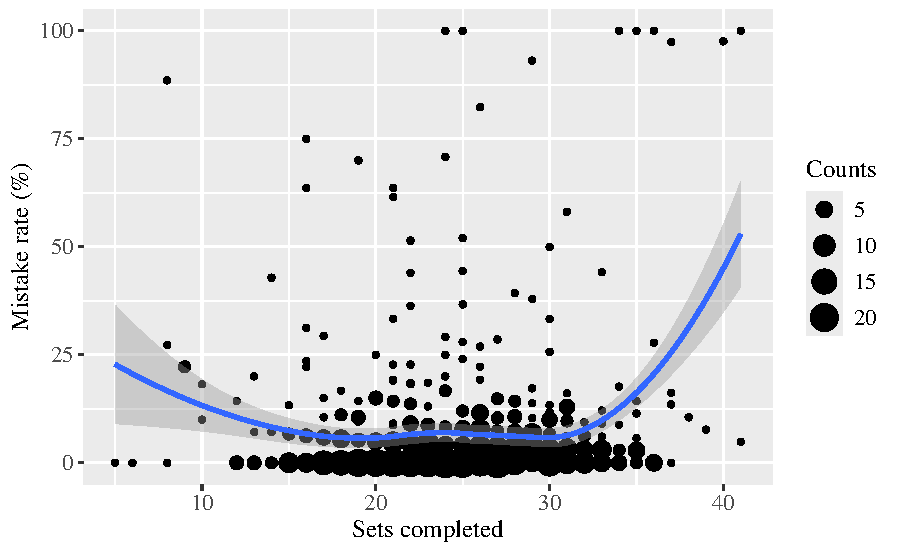
\includegraphics[width=0.75\linewidth,height=\textheight,keepaspectratio]{thesis-manuscript_files/figure-pdf/fig-effort-tradeoffs-1.pdf}

}

\subcaption{\label{fig-effort-tradeoffs-1}All data}

\centering{

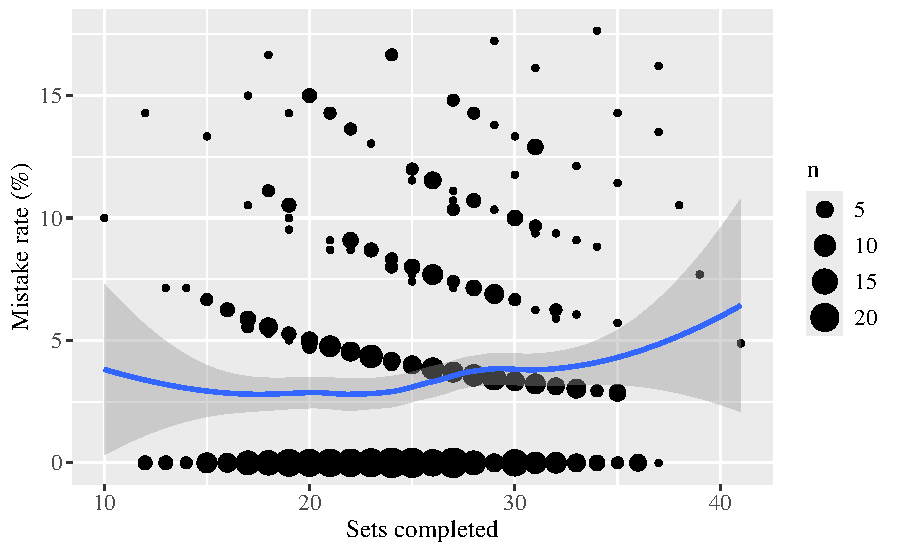
\includegraphics[width=0.75\linewidth,height=\textheight,keepaspectratio]{thesis-manuscript_files/figure-pdf/fig-effort-tradeoffs-2.pdf}

}

\subcaption{\label{fig-effort-tradeoffs-2}Without outliers}

}

\caption{\label{fig-effort-tradeoffs}Trade-offs between speed and
accuracy in the slider task}

\end{figure}%

\section{Results}\label{results}

\subsection{Econometric
specifications}\label{econometric-specifications}

The main analysis of reference point effects on effort exertion and
performance in the slider task uses regression (1), in which the
saturated model to be estimated is \[
log \frac {\mathbb{P}(Y_i = y_1)}{\mathbb{P}(Y_i = y_0)} = \beta_{1} + \beta_2 T_{2i} +\beta_3 T_{3i} +\beta_4 T_{4i} + \theta strict_i + \eta X_i + \varepsilon_i -(1)
\] \(Y_i\) is the categorical variable for whether subject \(i\)
achieved the targets, with four possible values: achieving both targets,
achieving the speed target only, achieving the accuracy target only, and
achieving none. Achieving none is set as the baseline (i.e.~\(y_0\)).
Since no subject achieved the speed target (and by consequence both
targets), there is only a single regression to run with \(y_1\)
corresponding to achievement of the accuracy target. Note this is based
on the \emph{recorded} mistake rate which depends on the assessment
criteria as well. \(T_{ji}\) corresponds to subject \(i\) being in
treatment group \(j\), with treatment 1 as the baseline (i.e.~omitted).
\(strict_i\) is a dummy variable for whether the subject was assessed by
the strict criterion. \(X_i\) is the vector of covariates and baseline
metrics from the demo task. The estimated coefficients are readily
interpretable as the increase in the log odds ratio of achieving the
accuracy target relative to achieving no targets, or equivalently an
increase in the odds ratio by the exponent \(e^{coefficient}\). This
maps nicely into treatment effects on the probability of target
achievement, which in turn measures the strength of reference point
effects.

The KR model predicts that the magnitude of the treatment coefficients
will be such that \(\beta_2 = \beta_4 < \beta_3\), whereas the appended
model predicts \(\beta_2 > \beta_3\) and \(\beta_2 > \beta_4\), and in
fact \(\beta_3\) and \(\beta_4\) may be insignificant. While I am
testing for multiple treatment effects, I do not consider them under the
same family of hypotheses, as the existence of probabilistic expectation
effects (\(\beta_2 \text{ vs } \beta_3\)) should not affect that of
cognitive complexity effects(\(\beta_2 \text{ vs } \beta_4\)), and both
are prerequisited on the existence of reference points
(\(\beta_2 \neq 0\)). In other words, they represent separate lines of
inquiry which can stand on their own.

To complement the above analysis, I estimated regression (2) and (3) to
examine treatment effects on mistake rate and sets completed
respectively, which elucidate shifts in effort towards/ away from each
dimension (intensive margin effects) even if they did not cause changes
in target achievement (extensive margin effects. \[
\begin{aligned}
& mistakerate_i = \gamma_1 + \gamma_2 T_{2i} + \gamma_3 T_{3i} + \gamma_4 T_{4i} + \phi strict_i + \psi X_i + \varepsilon_i -(2)
\\
& setscompleted_i = \delta_1 + \delta_2 T_{2i} + \delta_3 T_{3i} + \delta_4 T_{4i} + \mu strict_i + \nu X_i + \varepsilon_i -(3)
\end{aligned}
\] The two models' predictions on the treatment coefficients remain the
same as before. Note the predictions are now based on relative
magnitudes and sign-agnostic; given the data, the direction of reference
point effects will likely vary since accuracy performance in the control
already exceeds the set target for the treated groups but the inverse
holds for speed performance.

The above regression analysis was conducted for the pooled sample for
increased power, as well as separately on the lab sample and combined
class sample to check how effects may differ.

To further check experimental construct validity and that results are
indeed stemming from reference point effects, I ran regression (4) on
the pooled sample \[
log \frac {\mathbb{P}(Y_i = y_1)}{\mathbb{P}(Y_i = y_0)} = \pi_1 + \pi_2 T_{2i} + \pi_3 T_{3i} + \pi_4 T_{4i} + \tau_1 \lambda_i + \tau_2(T_{2i}*\lambda_i) + \rho strict_i + \sigma X_i + \varepsilon_i -(4)
\] \(\lambda_i\) is the subject's loss aversion level, measured in the
manner of Campos-Mercade et al. (2024), with subjects having been asked
to indicate the number of slider sets they are willing to complete under
fixed and random piece rates. While those responses were not
incentivised, they represent the best approximation given the budgetary
constraints of the experiment. If treatment 2 effects are truly coming
from the targets, they should increase in magnitude in the loss aversion
level, so \(\tau_2\) should be in the same sign as \(\pi_2\). I focus on
only treatment 2 for this verification since it is the most unambiguous
on reference point effects with respect to the different models'
predictions and to reduce the degrees of freedom exhausted. An analogue
is estimated in regression (5) and (6) with \(mistakerate_i\) and
\(setscompleted_i\) as the outcome variables respectively.

\subsection{Distributional comparisons of effort/ performance between
treatments}\label{distributional-comparisons-of-effort-performance-between-treatments}

Prior to the regression analysis, I conducted non-parametric comparisons
of sets completed and mistake rates in the slider task across treatment
groups. Figure~\ref{fig-slider-performance-distribution-comparison}
plots the cumulative distribution functions for the pooled sample. The
distribution of sets completed is very similar across treatments with
most subjects completing 25 sets and a rather symmetric spread around
it. Mistake rates are also quite similar, though treatment 3 is
dominated at low mistake rates up till 15\%. A joint Kruskal-Wallis test
between treatments of differences in medians indeed finds no significant
difference in sets completed (p-value = 0.11) but significant difference
in the latter (p-value = 0.013, which is still significant under
Bonferroni correction). Further pair-wise Kolmogorov distribution tests
of differences in distributions reveal that the significant difference
stems from treatment 3 (p-values = 0.0051 vs treatment 1, 0.049 vs
treatment 2, and 0.012 vs treatment 4). This could indicate attenuation
of reference point effects (if they exist), specifically in the accuracy
dimension, from the increased conflict between the effort dimensions in
treatment 3 where achieving both targets is more difficult.

Dissecting the sample into lab and class evinces that the differences
found above arise from the class sample
(Figure~\ref{fig-slider-performance-distribution-comparison-lab} and
Figure~\ref{fig-slider-performance-distribution-comparison-class} in
Appendix A1). Joint tests and pair-wise tests between treatments find no
significant differences in sets completed nor mistake rates in the lab
sample (the pair-wise test between treatments 2 and 4 does find
significant difference in sets completed with p-value = 0.047, but the
significance disappears after correction for multiple hypotheses
testing). Conversely in the class sample, the joint test finds
significant difference only for mistake rates and the pair-wise tests
find the same but only for treatment 3 compared to other groups,
paralleling the results in the pooled sample. In fact, this is likely
stemming from the macroeconomics class sample; its treatment 3 has the
highest mistake rate among all sub-sample-treatment combinations as seen
previously. Thus, whatever implied effects are not robust across
subsamples.

\begin{figure}

\centering{

\centering{

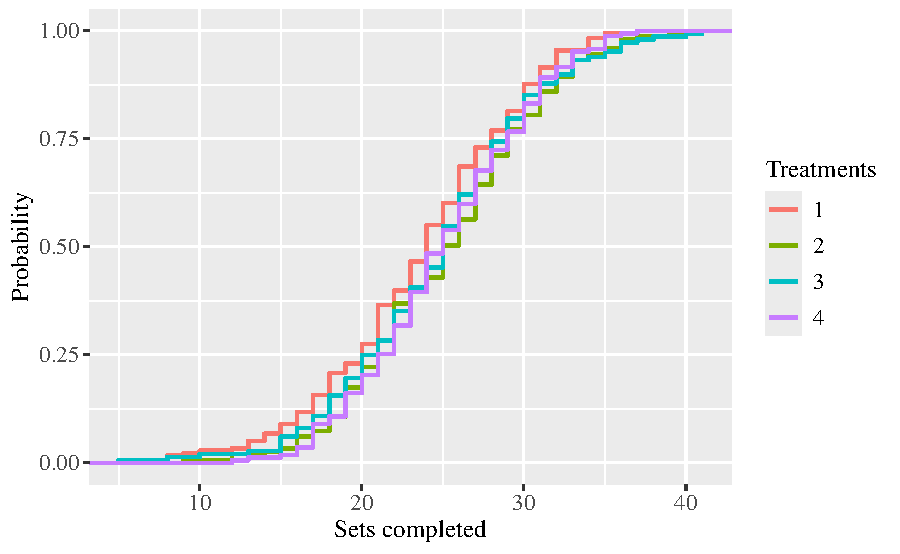
\includegraphics[width=0.75\linewidth,height=\textheight,keepaspectratio]{thesis-manuscript_files/figure-pdf/fig-slider-performance-distribution-comparison-1.pdf}

}

\subcaption{\label{fig-slider-performance-distribution-comparison-1}Sets
completed}

\centering{

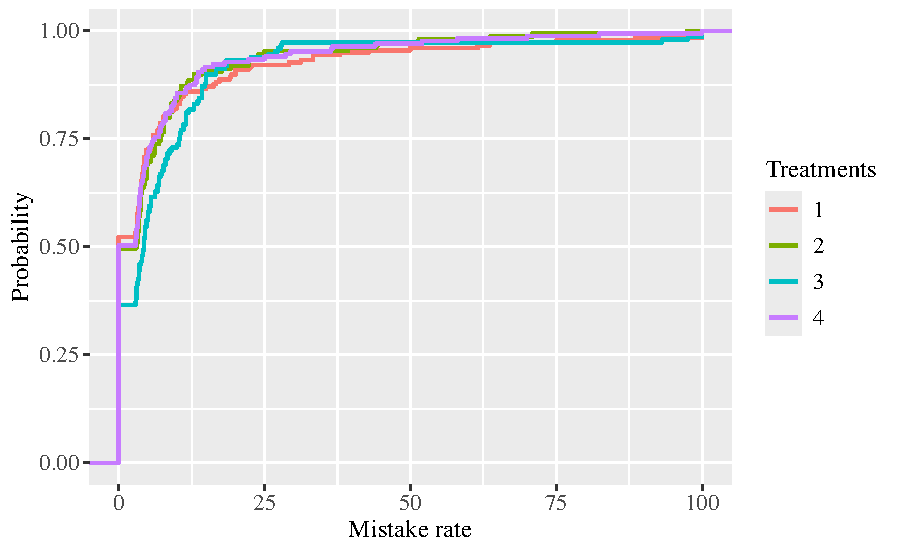
\includegraphics[width=0.75\linewidth,height=\textheight,keepaspectratio]{thesis-manuscript_files/figure-pdf/fig-slider-performance-distribution-comparison-2.pdf}

}

\subcaption{\label{fig-slider-performance-distribution-comparison-2}Mistake
rate}

}

\caption{\label{fig-slider-performance-distribution-comparison}Distributions
of key performance metrics in the slider task across treatments (pooled
sample)}

\end{figure}%

\subsection{Regression estimates of treatment effects on
effort}\label{regression-estimates-of-treatment-effects-on-effort}

Turning to a parametric estimation of treatment effects, regressions
(1), (2), and (3) are estimated on the pooled sample and presented in
Table~\ref{tbl-reg-target}, Table~\ref{tbl-reg-mistakes}, and
Table~\ref{tbl-reg-sets} respectively (full regression estimates in
Appendix A1). For each regression, model (1) regresses the outcome on
the treatments alone; model (2) controls for covariates; model (3)
controls for baseline performance in the demo task; and model (4)
controls for both. We see that the treatment coefficient estimates do
exhibit considerable variation in their magnitudes across the different
models in all regressions. Since there were some covariate imbalance
between treatments found in the sample, the estimates from the most
basic model (1) are likely least reliable. I focus on estimates from
models (3) and (4), which have the lowest Bayesian Information Criterion
and Akaike Information Criterion measures respectively in regression (1)
and the highest adjusted \(R^2\) values in regressions (2) and (3)
\footnote{The BIC more heavily penalises additional model parameters and
  hence rates model (4) worse despite it fitting the data better. The
  BIC is consistent in selecting the ``true'' model i.e.~it selects the
  true model as sample size approaches infinity, so it is appropriate
  for large sample sizes, though it is uncertain how well that holds
  here. Model (4) also suffers in regression (2) due to the high
  skewness of the outcome toward zero and high dimensionality of the
  regressors, causing problems with standard error computations.}. Note
model (3) also has the second lowest AIC in regression (1) and much
higher adjusted \(R^2\) values than model (2), meaning that the baseline
performance metrics do a relatively good job of predicting task effort
and performance, capturing most of the covariate effects and beyond.

Strikingly, regardless of the model used, all treatment effects on the
likelihood of achieving the accuracy target are negative, though not
significant, which seems to pose a paradox to hypothesized reference
point effects. However, note treatment effects on sets completed are
positive and significant at 5\% across the board. This is consistent
with the existence of reference point effects and subjects' inherent
prioritisation of accuracy (relative to the set targets). Consider that
subjects already had internally conceived targets for speed and
accuracy, which were mostly below 45 sets completed and below 10\%
mistake rate respectively; this is congruent with the mean performance
metrics in the control. Thus, externally setting targets of 45 sets
completed and 10\% mistake rate shifted subjects' focus away from their
internal targets to the external ones, inducing greater effort in the
speed dimension at the expense of the effort in the accuracy dimension.
This would produce the effects observed in regressions (1) and (2). The
insignificant results for the former likely reflects that subjects still
valued performance in accuracy much more than speed and hence were
unlikely to stray from the accuracy target. This is corroborated by
available survey responses to the question of why the subject did not
attempt to achieve both targets, with most citing that they focused on
accuracy more. A caveat is that treatment effects on mistake rate are
all negative also (i.e positive effect on accuracy), which could reflect
different effects at the extensive and intensive margins, but are also
less credible given the poorer data fit.

In this same vein of reasoning, now restricting focus to models (3) and
(4), we see that treatment 3 does show weaker reference point effects
than treatment 2, with smaller coefficient magnitudes in all
regressions. However, the difference in coefficients are not
significant: comparing effects on the likelihood of achieving the
accuracy target, p-value = 0.38 for model (3) and 0.88 for model (4);
comparing effects on mistake rate, p-value = 0.64 for model (3) and
unestimable for model (4); comparing effects on sets completed, p-value
= 0.34 for model (3) and 0.28 for model (4). This can be attributed to a
small base effect of the reference points, with treatment 2 only
increasing sets completed by 1.24 on average relative to the mean of
23.61 in the control, and decreasing the odds of achieving the accuracy
target by 0.58 times as opposed to the control increasing the odds by
10.59 times (based on model 4 estimates). Thus, any attenuation effects
would be even smaller (weakly) and harder to detect.

Conversely, treatment 4 does not show weaker reference point effects;
the magnitudes are smaller in regression (1) but larger in (2) and (3).
A considerable portion of respondents (107 out of 285) said that the
explanation of the targets did not make it easier for them to achieve
both targets nor make them more motivated to do so, so the treatments
may not have worked as intended. The mean time spent on instructions for
treatments 2 and 3 (59.34 and 52.32 seconds respectively) is much lower
than that for treatment 4 (143.30 seconds), suggesting that subjects may
not have actually digested the explanation of the targets in the former.

There are also some statistically significant covariate effects on
effort and performance \footnote{Covariate effects on mistake rates are
  not analysed since the saturated model is unstable and the model with
  only covariates has very poor fit.}. Those who studied undergraduate
economics are 2.44 times more likely to achieve the accuracy target,
though this could also be interpreted as class sample effects. Those
working in professional services are 8.94 times more likely to achieve
the accuracy target, but complete 1.5 sets less on average.
Surprisingly, using a mouse has no effect on achievement of the accuracy
target, likely because subjects' focus on this aspect more than
compensate for mouse usage, but does increase sets completed by 1 on
average. Female subjects complete 1 less set on average and Black
subjects complete 1.5 sets less on average. Some significant effects for
income brackets are observed but there are no meaningful patterns.
Having an education level of below a high school diploma critically
reduces sets completed by 3 but it is likely due to pure chance given
there is only one observation in this category.

The treatment effects found above are somewhat robust to estimation by
subsamples (tables in Appendix A1). The reference point effects in
treatment 2 stay similar in the lab and class samples, with negative
effects on likelihood of achieving the accuracy target and positive
effects on sets completed, although the latter are no longer
significant, likely due to smaller sample size and noisier estimates
(much larger standard deviations). The effect sizes of treatment 4
relative to treatment 2 remain ambiguous in both subsamples. Treatment 3
effects for the lab sample are congruent with the pooled sample, being
less negative for accuracy target achievements and less positive for
sets completed relative to treatment 2, with significant differences
found for the former (p-values = 0.024 for model (3) and 0.038 for model
(4)). The main difference lies in treatment 3 effects for class sample,
which show more negative effects for accuracy target achievement, though
they are still less positive for sets completed; no differences are
significant. The discrepancy is plausibly attributed to sampling error
in the macroeconomic class sample whose treatment 3 had the highest
mistake rate.

\begin{table}

\centering{

\begin{center}
\begin{tabular}{l c c c c}
\hline
 & \multicolumn{4}{c}{Log odds of achieving accuracy target} \\
\cline{2-5}
 & Model 1 & Model 2 & Model 3 & Model 4 \\
\hline
(Intercept)                     & $3.41^{***}$  & $3.00^{***}$  & $3.29^{***}$  & $2.36^{*}$    \\
                                & $(0.43)$      & $(0.76)$      & $(0.68)$      & $(0.99)$      \\
treatment2                      & $-0.53$       & $-0.35$       & $-0.76$       & $-0.54$       \\
                                & $(0.38)$      & $(0.44)$      & $(0.40)$      & $(0.46)$      \\
treatment3                      & $-0.52$       & $-0.57$       & $-0.42$       & $-0.47$       \\
                                & $(0.29)$      & $(0.33)$      & $(0.32)$      & $(0.37)$      \\
treatment4                      & $-0.03$       & $-0.12$       & $-0.08$       & $-0.08$       \\
                                & $(0.43)$      & $(0.47)$      & $(0.46)$      & $(0.51)$      \\
\hline
Baselines & No & No & Yes & Yes \\
Covariates & No & Yes & No & Yes \\
\hline
AIC                             & $474.96$      & $420.88$      & $419.62$      & $381.34$      \\
BIC                             & $497.28$      & $537.20$      & $455.34$      & $510.59$      \\
Log Likelihood                  & $-232.48$     & $-183.44$     & $-201.81$     & $-160.67$     \\
Num. obs.                       & $642$         & $549$         & $642$         & $549$         \\
\hline
\multicolumn{5}{l}{\scriptsize{$^{***}p<0.001$; $^{**}p<0.01$; $^{*}p<0.05$}}
\end{tabular}
\label{table:coefficients}
\end{center}

}

\caption{\label{tbl-reg-target}Treatment effects on accuracy target
achivement likelihood (pooled sample)}

\end{table}%

\begin{table}

\centering{

\begin{center}
\begin{tabular}{l c c c c}
\hline
 & \multicolumn{4}{c}{Mistake rate} \\
\cline{2-5}
 & Model 1 & Model 2 & Model 3 & Model 4 \\
\hline
(Intercept)                     & $8.96^{***}$ & $11.80^{***}$ & $7.66^{**}$  & $10.59$ \\
                                & $(1.97)$     & $(2.95)$      & $(2.69)$     & $$      \\
treatment2                      & $-2.22$      & $-3.13$       & $-1.75$      & $-3.16$ \\
                                & $(1.90)$     & $(1.86)$      & $(1.64)$     & $$      \\
treatment3                      & $0.30$       & $-0.45$       & $-1.07$      & $-1.41$ \\
                                & $(1.91)$     & $(1.82)$      & $(1.50)$     & $$      \\
treatment4                      & $-2.37$      & $-1.91$       & $-2.20$      & $-2.13$ \\
                                & $(1.94)$     & $(2.04)$      & $(1.72)$     & $$      \\
\hline
Baselines & No & No & Yes & Yes \\
Covariates & No & Yes & No & Yes \\
\hline
R$^2$                           & $0.00$       & $0.08$        & $0.27$       & $0.29$  \\
Adj. R$^2$                      & $-0.00$      & $0.03$        & $0.26$       & $0.25$  \\
Num. obs.                       & $642$        & $549$         & $642$        & $549$   \\
RMSE                            & $15.62$      & $14.93$       & $13.43$      & $13.12$ \\
\hline
\multicolumn{5}{l}{\scriptsize{$^{***}p<0.001$; $^{**}p<0.01$; $^{*}p<0.05$}}
\end{tabular}
\label{table:coefficients}
\end{center}

}

\caption{\label{tbl-reg-mistakes}Treatment effects on mistake rate
(pooled sample)}

\end{table}%

\begin{table}

\centering{

\begin{center}
\begin{tabular}{l c c c c}
\hline
 & \multicolumn{4}{c}{Sets completed} \\
\cline{2-5}
 & Model 1 & Model 2 & Model 3 & Model 4 \\
\hline
(Intercept)                     & $23.52^{***}$ & $22.60^{***}$ & $8.41^{***}$ & $8.89^{***}$  \\
                                & $(0.79)$      & $(1.23)$      & $(0.97)$     & $(1.28)$      \\
treatment2                      & $1.69^{*}$    & $1.60^{*}$    & $1.46^{*}$   & $1.24^{*}$    \\
                                & $(0.81)$      & $(0.77)$      & $(0.57)$     & $(0.59)$      \\
treatment3                      & $1.15$        & $0.74$        & $0.95$       & $0.66$        \\
                                & $(0.69)$      & $(0.68)$      & $(0.49)$     & $(0.52)$      \\
treatment4                      & $1.53$        & $1.36$        & $1.59^{**}$  & $1.36^{*}$    \\
                                & $(0.80)$      & $(0.76)$      & $(0.61)$     & $(0.63)$      \\
\hline
Baselines & No & No & Yes & Yes \\
Covariates & No & Yes & No & Yes \\
\hline
R$^2$                           & $0.01$        & $0.22$        & $0.46$       & $0.53$        \\
Adj. R$^2$                      & $0.01$        & $0.18$        & $0.45$       & $0.50$        \\
Num. obs.                       & $642$         & $549$         & $642$        & $549$         \\
RMSE                            & $5.78$        & $5.30$        & $4.29$       & $4.13$        \\
\hline
\multicolumn{5}{l}{\tiny{$^{***}p<0.001$; $^{**}p<0.01$; $^{*}p<0.05$}}
\end{tabular}
\label{table:coefficients}
\end{center}

}

\caption{\label{tbl-reg-sets}Treatment effects on sets completed (pooled
sample)}

\end{table}%

\subsection{Verification of reference point
effects}\label{verification-of-reference-point-effects}

A final robustness check of the purported reference point effects is
done by interacting treatment effects with loss aversion levels in the
pooled sample.

Loss aversion levels were estimated following Campos-Mercade et al.
(2024) which assume KR reference-dependent preferences. In the post-task
survey, subjects were asked to indicate the number of correctly
completed sets they were willing to do under different payment
structures, which consisted of seven different fixed piece rates and
seven different random piece rates. The random piece rate paid out
either a high piece rate or low piece rate with equal probabilities, and
each had an expected payment equal to one of the fixed piece rates.
Assuming an effort cost function of
\(c(e) = \frac {1}{\alpha + \omega} e^\omega\) as in the original paper
and based upon Augenblick and Rabin (2019), we obtain the reduced form
approximation \[
\begin{aligned}
& log(e_i) \approx J_i + K_i log(\bar{w}) - L_i \frac{\Delta w}{\bar w} \\
& \text{Where} \\
& J_i = \frac {log(\alpha_i)}{\omega_i - 1}; \space K_i = \frac {1}{\omega_i - 1}; \space L_i = \frac {\lambda_i -1}{4(\omega_i - 1)} = \frac {1}{4} K_i (\lambda_i -1) 
\end{aligned}
\] \(\bar w\) is the average piece rate, which is just equal to the
piece rate for fixed payments, whereas \(\Delta w = w_h - w_l\) is the
piece rate spread where \(w_h\) is the high piece rate and \(w_l\) is
the low piece rate paid out in random payments, and equal to zero for
fixed payments. Recall that \(\lambda_i\) is the loss aversion
parameter, so \(L_i\) acts as its reduced form estimate. Given the
approximation holds with some mean zero error term, we can estimate the
equation using OLS regression.\footnote{Estimates of \(\lambda_i\) had
  to be top-coded at 4.33 given the maximum
  \(\frac{\Delta w}{\bar w} = 1.2\) in the survey, otherwise the
  logarithms in the approximated equation below will be undefined. \[
  log(e_i) = J_i + K_i log(\bar{w}) + K_i log(1 + 0.25 (1 - \lambda_i) \frac{\Delta w}{\bar w})
  \] Estimates were also bottom-coded at 0 as negative values are
  difficult to interpret (would imply utility gains from losses).}

After obtaining structural estimates of the loss aversion parameters, I
run regressions (4), (5) and (6) using just models (3) and (4) now,
omitting The results in Table~\ref{tbl-reg-target-la},
Table~\ref{tbl-reg-mistakes-la}, and Table~\ref{tbl-reg-sets-la} detract
from the reference point effects posited above as the coefficient on the
interaction term between treatment 2 and the loss aversion level is
positive when the outcome is the log odds of accuracy target achievement
and negative when the outcome is sets completed, which contradicts the
hypothesis that more loss averse individuals should be more affected by
the set targets to induce greater effort in speed and less in accuracy.

A caveat is that the loss aversion estimation could be unreliable since
it was unincentivised and hence the reports are likely to suffer from
hypothetical bias. Almost half of the raw estimates (248 out of 503) lie
beyond the upper and lower bounds allowed by the estimation, with a
considerable portion (176) having negative loss aversion parameters
before top and bottom-coding adjustments. Data quality aside, the
interaction between loss aversion and treatment effects is also
ambiguous, since loss aversion can be with respect to both internally
conceived targets and externally set ones, hence it could either
counteract or reinforce the suggested reference point effects. These
complications in interpretation arise due to the different directions of
effect exerted by the reference points in each effort/ performance
dimension.

Nevertheless, in accordance with the original analysis plan and
hypothesis, this exercise refutes that treatment effects can be
attributed to reference points, hence the (in)validation of both models'
predictions are inconclusive. Since treatment effects are dubious and
not significant, this was a moot point, I do not proceed with
heterogeneity analysis.

\begin{table}

\centering{

\begin{center}
\begin{tabular}{l c c}
\hline
 & \multicolumn{2}{c}{Log odds of achieving accuracy target} \\
\cline{2-3}
 & Model 3 & Model 4 \\
\hline
(Intercept)                     & $3.88^{***}$  & $3.12^{*}$    \\
                                & $(0.84)$      & $(1.21)$      \\
treatment2                      & $-1.09$       & $-1.25$       \\
                                & $(0.59)$      & $(0.68)$      \\
treatment3                      & $-0.33$       & $-0.39$       \\
                                & $(0.38)$      & $(0.43)$      \\
treatment4                      & $-0.37$       & $-0.29$       \\
                                & $(0.52)$      & $(0.57)$      \\
criterionstrict                 & $-2.35^{***}$ & $-2.61^{***}$ \\
                                & $(0.52)$      & $(0.59)$      \\
lambda\_i\_adj                  & $-0.11$       & $-0.13$       \\
                                & $(0.10)$      & $(0.12)$      \\
treatment2\_lambda\_i\_adj      & $0.36$        & $0.42$        \\
                                & $(0.28)$      & $(0.30)$      \\
\hline
Baselines & Yes & Yes \\
Covariates & No & Yes \\
\hline
AIC                             & $309.89$      & $302.22$      \\
BIC                             & $352.10$      & $430.29$      \\
Log Likelihood                  & $-144.95$     & $-120.11$     \\
Num. obs.                       & $503$         & $460$         \\
\hline
\multicolumn{3}{l}{\scriptsize{$^{***}p<0.001$; $^{**}p<0.01$; $^{*}p<0.05$}}
\end{tabular}
\label{table:coefficients}
\end{center}

}

\caption{\label{tbl-reg-target-la}Treatment effects on target
achievement interacted with loss aversion}

\end{table}%

\begin{table}

\centering{

\begin{center}
\begin{tabular}{l c c}
\hline
 & \multicolumn{2}{c}{Mistake rate} \\
\cline{2-3}
 & Model 3 & Model 4 \\
\hline
(Intercept)                     & $6.68^{*}$   & $8.99^{*}$   \\
                                & $(2.67)$     & $(4.11)$     \\
treatment2                      & $-2.51$      & $-1.98$      \\
                                & $(1.91)$     & $(1.91)$     \\
treatment3                      & $-1.11$      & $-1.06$      \\
                                & $(1.58)$     & $(1.58)$     \\
treatment4                      & $-1.84$      & $-1.39$      \\
                                & $(1.95)$     & $(2.03)$     \\
criterionstrict                 & $-2.28$      & $-1.50$      \\
                                & $(1.32)$     & $(1.15)$     \\
lambda\_i\_adj                  & $-0.00$      & $-0.02$      \\
                                & $(0.50)$     & $(0.54)$     \\
treatment2\_lambda\_i\_adj      & $-0.71$      & $-0.92$      \\
                                & $(0.73)$     & $(0.76)$     \\
\hline
Baselines & Yes & Yes \\
Covariates & No & Yes \\
\hline
R$^2$                           & $0.23$       & $0.27$       \\
Adj. R$^2$                      & $0.22$       & $0.22$       \\
Num. obs.                       & $503$        & $460$        \\
RMSE                            & $12.71$      & $12.54$      \\
\hline
\multicolumn{3}{l}{\scriptsize{$^{***}p<0.001$; $^{**}p<0.01$; $^{*}p<0.05$}}
\end{tabular}
\label{table:coefficients}
\end{center}

}

\caption{\label{tbl-reg-mistakes-la}Treatment effects on mistake rate
interacted with loss aversion}

\end{table}%

\begin{table}

\centering{

\begin{center}
\begin{tabular}{l c c}
\hline
 & \multicolumn{2}{c}{Sets completed} \\
\cline{2-3}
 & Model 3 & Model 4 \\
\hline
(Intercept)                     & $8.21^{***}$  & $9.31^{***}$ \\
                                & $(1.11)$      & $(1.43)$     \\
treatment2                      & $1.28$        & $1.07$       \\
                                & $(0.78)$      & $(0.83)$     \\
treatment3                      & $0.71$        & $0.50$       \\
                                & $(0.56)$      & $(0.61)$     \\
treatment4                      & $1.45^{*}$    & $1.40^{*}$   \\
                                & $(0.70)$      & $(0.71)$     \\
criterionstrict                 & $0.15$        & $0.26$       \\
                                & $(0.53)$      & $(0.53)$     \\
lambda\_i\_adj                  & $0.11$        & $0.12$       \\
                                & $(0.14)$      & $(0.14)$     \\
treatment2\_lambda\_i\_adj      & $-0.05$       & $-0.06$      \\
                                & $(0.26)$      & $(0.26)$     \\
\hline
Baselines & Yes & Yes \\
Covariates & No & Yes \\
\hline
R$^2$                           & $0.46$        & $0.51$       \\
Adj. R$^2$                      & $0.45$        & $0.48$       \\
Num. obs.                       & $503$         & $460$        \\
RMSE                            & $4.29$        & $4.18$       \\
\hline
\multicolumn{3}{l}{\scriptsize{$^{***}p<0.001$; $^{**}p<0.01$; $^{*}p<0.05$}}
\end{tabular}
\label{table:coefficients}
\end{center}

}

\caption{\label{tbl-reg-sets-la}Treatment effects on sets completed
interacted with loss aversion}

\end{table}%

\newpage

\section{Conclusion}\label{conclusion}

This paper has investigated potential interaction effects between
multi-dimensional reference points, specifically the attenuation of
conflicting reference points due to low probabilistic expectations of
concurrently achieving them and/ or cognitive complexity in reconciling
them. The experiment found some weak evidence for such effects, but they
were mostly statistically insignificant and not robust to sampling
differences. They also failed the construct validity check of whether
the effects are indeed stemming from reference points (though the
verification method itself was problematic due to unincentivised
responses).

Overall, budgetary and time constraints led to less than ideal
experimental design which failed to offer conclusive insights on how
humans aggregate across reference points in multiple dimensions, with
neither strong support for the original or augmented KR model. However,
the experimental results do highlight the dynamics between internally
conceived and externally imposed targets in reference point formation,
which signals a potential new avenue for research.

\newpage

\section{Bibliography}\label{bibliography}

\phantomsection\label{refs}
\begin{CSLReferences}{1}{0}
\bibitem[\citeproctext]{ref-abeler.2011.referencepoints}
Abeler, Johannes, Armin Falk, Lorenz Goette, and David Huffman. 2011.
{``Reference {Points} and {Effort Provision}.''} \emph{American Economic
Review} 101 (2): 470--92. \url{https://doi.org/10.1257/aer.101.2.470}.

\bibitem[\citeproctext]{ref-augenblick.2019.experimenttime}
Augenblick, Ned, and Matthew Rabin. 2019. {``An {Experiment} on {Time
Preference} and {Misprediction} in {Unpleasant Tasks}.''} \emph{The
Review of Economic Studies} 86 (3): 941--75.
\url{https://doi.org/10.1093/restud/rdy019}.

\bibitem[\citeproctext]{ref-bai.2022.optimalitymatchedpair}
Bai, Yuehao. 2022. {``Optimality of {Matched-Pair Designs} in
{Randomized Controlled Trials}.''} \emph{American Economic Review} 112
(12): 3911--40. \url{https://doi.org/10.1257/aer.20201856}.

\bibitem[\citeproctext]{ref-bell.1982.regretdecision}
Bell, David E. 1982. {``Regret in {Decision Making} Under
{Uncertainty}.''} \emph{Operations Research} 30 (5): 961--81.
\url{https://doi.org/10.1287/opre.30.5.961}.

\bibitem[\citeproctext]{ref-bell.1985.disappointmentdecision}
---------. 1985. {``Disappointment in {Decision Making Under
Uncertainty}.''} \emph{Operations Research} 33 (1): 1--27.
\url{https://doi.org/10.1287/opre.33.1.1}.

\bibitem[\citeproctext]{ref-campos-mercade.2024.gustibusdisputes}
Campos-Mercade, Pol, Lorenz Goette, Thomas Graeber, Alexandre Kellogg,
and Charles Sprenger. 2024. {``De {Gustibus} and {Disputes} about
{Reference Dependence}.''} R\textbackslash\&\{\{R\}\} at \{\{The
Review\}\} of \{\{Economic Studies\}\}.

\bibitem[\citeproctext]{ref-crawford.2011.newyork}
Crawford, Vincent P, and Juanjuan Meng. 2011. {``New {York City Cab
Drivers}' {Labor Supply Revisited}: {Reference-Dependent Preferences}
with {Rational-Expectations Targets} for {Hours} and {Income}.''}
\emph{American Economic Review} 101 (5): 1912--32.
\url{https://doi.org/10.1257/aer.101.5.1912}.

\bibitem[\citeproctext]{ref-genesove.2001.lossaversion}
Genesove, D., and C. Mayer. 2001. {``Loss {Aversion} and {Seller
Behavior}: {Evidence} from the {Housing Market}.''} \emph{The Quarterly
Journal of Economics} 116 (4): 1233--60.
\url{https://doi.org/10.1162/003355301753265561}.

\bibitem[\citeproctext]{ref-gul.1991.theorydisappointment}
Gul, Faruk. 1991. {``A {Theory} of {Disappointment Aversion}.''}
\emph{Econometrica : Journal of the Econometric Society} 59 (3):
667--86. \url{https://doi.org/10.2307/2938223}.

\bibitem[\citeproctext]{ref-harrison.2009.riskattitudes}
Harrison, Glenn W., Morten I. Lau, and E. Elisabet Rutström. 2009.
{``Risk Attitudes, Randomization to Treatment, and Self-Selection into
Experiments.''} \emph{Journal of Economic Behavior \& Organization} 70
(3): 498--507. \url{https://doi.org/10.1016/j.jebo.2008.02.011}.

\bibitem[\citeproctext]{ref-hayes.1984.restoringour}
Hayes, Robert H. 1984. \emph{Restoring Our Competitive Edge :
{Competing} Through Manufacturing}. Edited by Steven C. Wheelwright. New
York: Wiley.

\bibitem[\citeproctext]{ref-hayes.1978.howshould}
Hayes, Robert H, and Roger W Schmenner. 1978. {``How Should You Organize
Manufacturing.''} \emph{Harvard Business Review} 56 (1): 105--18.

\bibitem[\citeproctext]{ref-heath.1999.goalsreference}
Heath, Chip, Richard P. Larrick, and George Wu. 1999. {``Goals as
{Reference Points}.''} \emph{Cognitive Psychology} 38 (1): 79--109.
\url{https://doi.org/10.1006/cogp.1998.0708}.

\bibitem[\citeproctext]{ref-kahneman.1990.experimentaltests}
Kahneman, Daniel, Jack L. Knetsch, and Richard H. Thaler. 1990.
{``Experimental {Tests} of the {Endowment Effect} and the {Coase
Theorem}.''} \emph{Journal of Political Economy} 98 (6): 1325--48.
\url{https://doi.org/10.1086/261737}.

\bibitem[\citeproctext]{ref-kahneman.1979.prospecttheory}
Kahneman, Daniel, and Amos Tversky. 1979. {``Prospect {Theory}: {An
Analysis} of {Decision} Under {Risk}.''} \emph{Econometrica : Journal of
the Econometric Society} 47 (2): 263.
\url{https://doi.org/10.2307/1914185}.

\bibitem[\citeproctext]{ref-koszegi.2006.modelreferencedependenta}
Koszegi, B., and M. Rabin. 2006. {``A {Model} of {Reference-Dependent
Preferences}.''} \emph{The Quarterly Journal of Economics} 121 (4):
1133--65. \url{https://doi.org/10.1093/qje/121.4.1133}.

\bibitem[\citeproctext]{ref-loomes.1982.regrettheory}
Loomes, Graham, and Robert Sugden. 1982. {``Regret {Theory}: {An
Alternative Theory} of {Rational Choice Under Uncertainty}.''} \emph{The
Economic Journal} 92 (368): 805. \url{https://doi.org/10.2307/2232669}.

\bibitem[\citeproctext]{ref-loomes.1986.disappointmentdynamic}
---------. 1986. {``Disappointment and {Dynamic Consistency} in {Choice}
Under {Uncertainty}.''} \emph{The Review of Economic Studies} 53 (2):
271--82. \url{https://doi.org/10.2307/2297651}.

\bibitem[\citeproctext]{ref-plott.2005.willingnesspay}
Plott, Charles R, and Kathryn Zeiler. 2005. {``The {Willingness} to
{Pay}--{Willingness} to {Accept Gap}, the {`{Endowment Effect},'}
{Subject Misconceptions}, and {Experimental Procedures} for {Eliciting
Valuations}.''} \emph{American Economic Review} 95 (3): 530--45.
\url{https://doi.org/10.1257/0002828054201387}.

\bibitem[\citeproctext]{ref-skinner.1974.focusedfactory}
Skinner, Wickham. 1974. {``The Focused Factory.''} \emph{Harvard
Business Review} 52: 113--21.

\bibitem[\citeproctext]{ref-skinner.1996.manufacturingstrategy}
---------. 1996. {``{MANUFACTURING STRATEGY ON THE} {`{S}'} {CURVE}.''}
\emph{Production and Operations Management} 5 (1): 3--14.
\url{https://doi.org/10.1111/j.1937-5956.1996.tb00381.x}.

\bibitem[\citeproctext]{ref-swamidass.2000.focusedfactory}
Swamidass, Paul M., and Neil R. Darlow. 2000. {``{FOCUSED FACTORY}.''}
In \emph{Encyclopedia of {Production} and {Manufacturing Management}},
edited by P. M. Swamidass, 219--24. New York, NY: Springer US.
\url{https://doi.org/10.1007/1-4020-0612-8_355}.

\bibitem[\citeproctext]{ref-tversky.1991.lossaversion}
Tversky, A., and D. Kahneman. 1991. {``Loss {Aversion} in {Riskless
Choice}: {A Reference-Dependent Model}.''} \emph{The Quarterly Journal
of Economics} 106 (4): 1039--61. \url{https://doi.org/10.2307/2937956}.

\bibitem[\citeproctext]{ref-vonrechenberg.2016.goalsreference}
Von Rechenberg, Tobias, Dominik Gutt, and Dennis Kundisch. 2016.
{``Goals as {Reference Points}: {Empirical Evidence} from a {Virtual
Reward System}.''} \emph{Decision Analysis} 13 (2): 153--71.
\url{https://doi.org/10.1287/deca.2016.0331}.

\end{CSLReferences}

\newpage

\section{Acknowledgements}\label{acknowledgements}

Special thanks to

\begin{itemize}
\tightlist
\item
  Professor Fulya Ersoy for advising this thesis, including refining the
  research idea and experimental design, obtaining IRB approval, and
  providing feedback on my writing
\item
  Professors Min Sok Lee and Kanit (Ken) Kuevibulvanich for helping to
  run the experiment with their classes
\item
  The RF-CDR team for helping to run the experiment at their lab, namely

  \begin{itemize}
  \tightlist
  \item
    Nina Semushina
  \item
    Lucia Agajanian
  \item
    Justin Daugherty
  \item
    Akshaj Dwivedula
  \item
    Pablo Paucar
  \item
    Angelysse Madsen
  \item
    Adam Vargas
  \item
    Kaushal Addanki
  \item
    Charlotte Parque
  \end{itemize}
\item
  My friends Elliot Lin, Lim Mian, Nour Abdelbaki and others who helped
  to test and debug the survey and provided moral support
\end{itemize}

\newpage

\section{Appendix}\label{appendix}

\subsection{A1. Figures and tables}\label{a1.-figures-and-tables}

\begin{figure}[H]

\centering{

\centering{

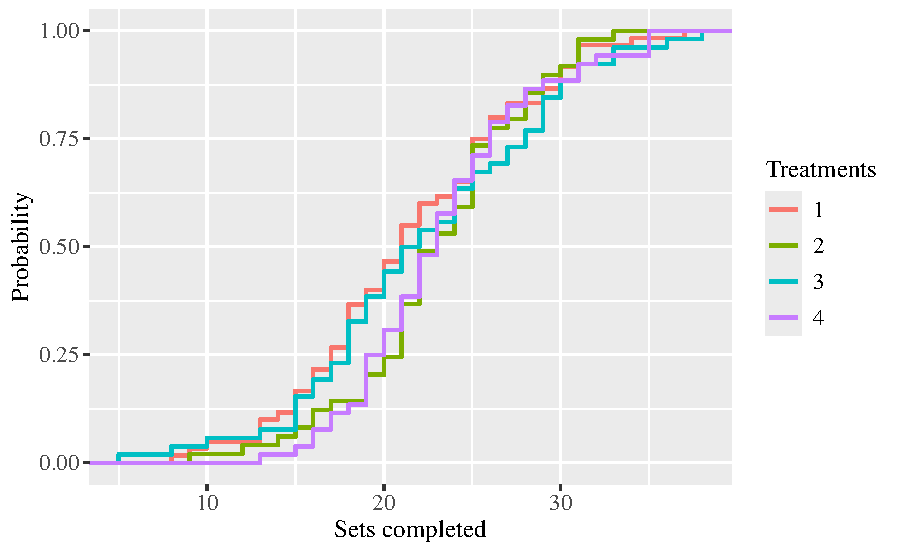
\includegraphics[width=0.75\linewidth,height=\textheight,keepaspectratio]{thesis-manuscript_files/figure-pdf/fig-slider-performance-distribution-comparison-lab-1.pdf}

}

\subcaption{\label{fig-slider-performance-distribution-comparison-lab-1}Sets
completed}

\centering{

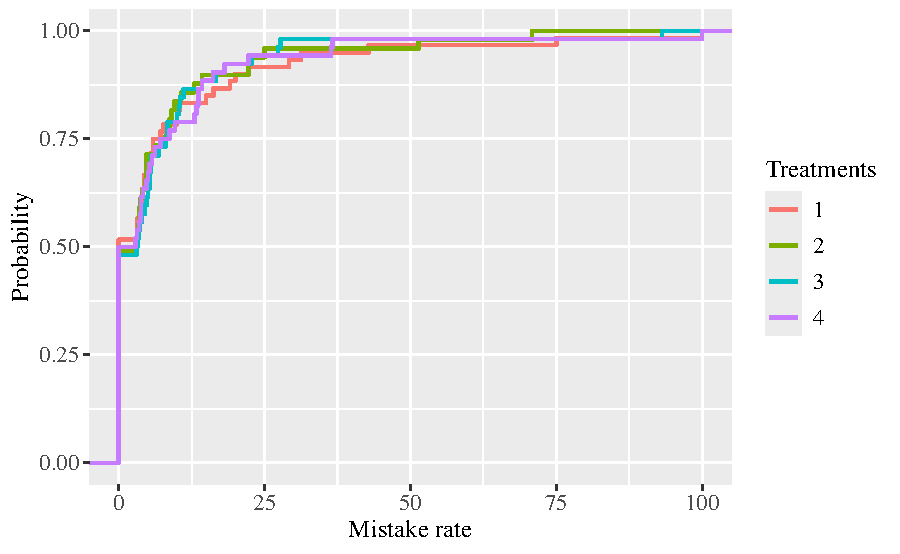
\includegraphics[width=0.75\linewidth,height=\textheight,keepaspectratio]{thesis-manuscript_files/figure-pdf/fig-slider-performance-distribution-comparison-lab-2.pdf}

}

\subcaption{\label{fig-slider-performance-distribution-comparison-lab-2}Mistake
rate}

}

\caption{\label{fig-slider-performance-distribution-comparison-lab}Distributions
of key performance metrics in the slider task across treatments (lab
sample)}

\end{figure}%

\begin{figure}

\centering{

\centering{

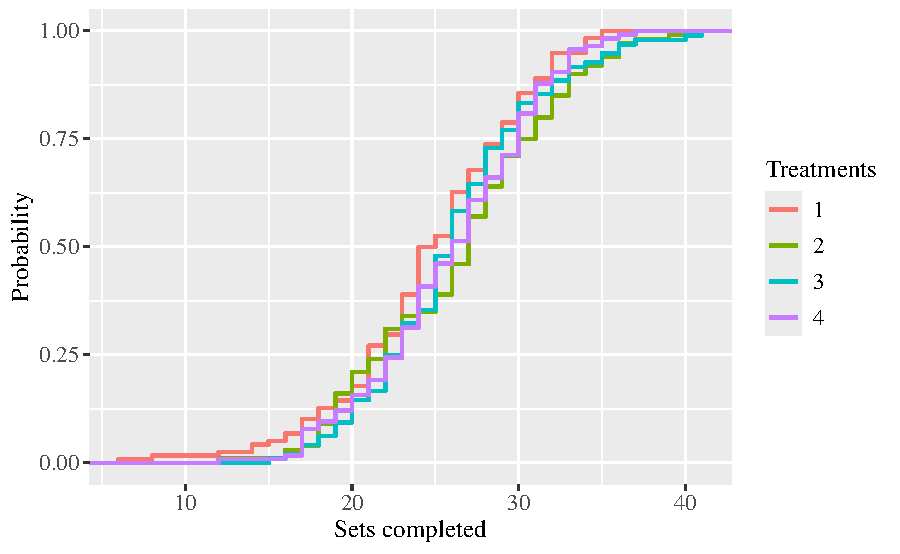
\includegraphics[width=0.75\linewidth,height=\textheight,keepaspectratio]{thesis-manuscript_files/figure-pdf/fig-slider-performance-distribution-comparison-class-1.pdf}

}

\subcaption{\label{fig-slider-performance-distribution-comparison-class-1}Sets
completed}

\centering{

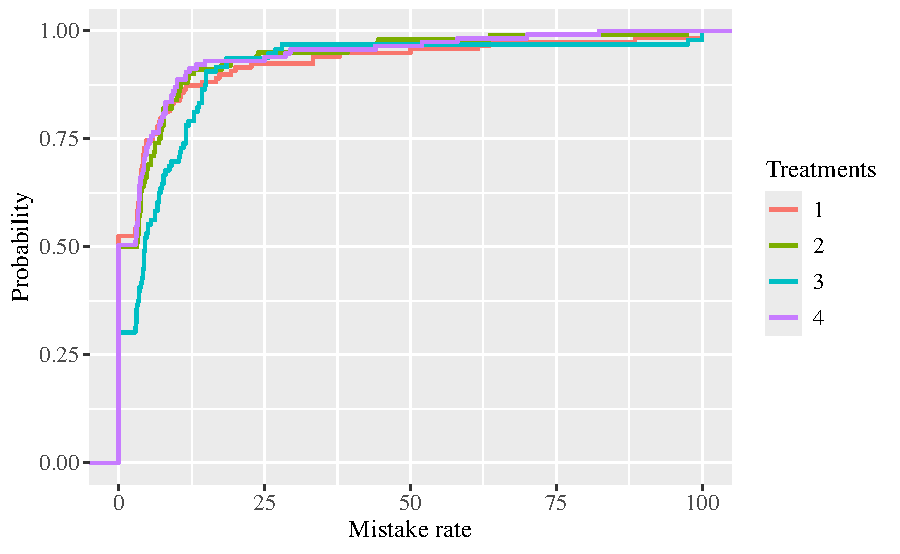
\includegraphics[width=0.75\linewidth,height=\textheight,keepaspectratio]{thesis-manuscript_files/figure-pdf/fig-slider-performance-distribution-comparison-class-2.pdf}

}

\subcaption{\label{fig-slider-performance-distribution-comparison-class-2}Mistake
rate}

}

\caption{\label{fig-slider-performance-distribution-comparison-class}Distributions
of key performance metrics in the slider task across treatments (class
sample)}

\end{figure}%

\begin{table}

\centering{

\scriptsize
\begin{center}
\begin{tabular}{l c c c c}
\hline
 & \multicolumn{4}{c}{Log odds of achieving accuracy target} \\
\cline{2-5}
 & Model 1 & Model 2 & Model 3 & Model 4 \\
\hline
(Intercept)                     & $3.41^{***}$  & $3.00^{***}$  & $3.29^{***}$  & $2.36^{*}$    \\
                                & $(0.43)$      & $(0.76)$      & $(0.68)$      & $(0.99)$      \\
treatment2                      & $-0.53$       & $-0.35$       & $-0.76$       & $-0.54$       \\
                                & $(0.38)$      & $(0.44)$      & $(0.40)$      & $(0.46)$      \\
treatment3                      & $-0.52$       & $-0.57$       & $-0.42$       & $-0.47$       \\
                                & $(0.29)$      & $(0.33)$      & $(0.32)$      & $(0.37)$      \\
treatment4                      & $-0.03$       & $-0.12$       & $-0.08$       & $-0.08$       \\
                                & $(0.43)$      & $(0.47)$      & $(0.46)$      & $(0.51)$      \\
criterionstrict                 & $-1.81^{***}$ & $-1.97^{***}$ & $-2.22^{***}$ & $-2.31^{***}$ \\
                                & $(0.38)$      & $(0.44)$      & $(0.42)$      & $(0.48)$      \\
genderFemale                    &               & $0.07$        &               & $0.04$        \\
                                &               & $(0.29)$      &               & $(0.31)$      \\
genderNon-binary                &               & $16.05$       &               & $15.37$       \\
                                &               & $(1329.79)$   &               & $(1341.41)$   \\
raceAsian                       &               & $0.36$        &               & $0.21$        \\
                                &               & $(0.32)$      &               & $(0.34)$      \\
raceBlack                       &               & $0.31$        &               & $0.21$        \\
                                &               & $(0.51)$      &               & $(0.55)$      \\
raceHispanic                    &               & $1.05$        &               & $0.89$        \\
                                &               & $(0.60)$      &               & $(0.62)$      \\
raceMixed                       &               & $-0.50$       &               & $-0.22$       \\
                                &               & $(0.58)$      &               & $(0.72)$      \\
income25,000 - 49,999           &               & $-0.18$       &               & $-0.39$       \\
                                &               & $(0.70)$      &               & $(0.73)$      \\
income50,000 - 74,999           &               & $-0.68$       &               & $-0.59$       \\
                                &               & $(0.65)$      &               & $(0.70)$      \\
income75,000 - 119,999          &               & $-1.09$       &               & $-1.26^{*}$   \\
                                &               & $(0.59)$      &               & $(0.64)$      \\
income120,000 - 199,999         &               & $0.44$        &               & $0.20$        \\
                                &               & $(0.69)$      &               & $(0.73)$      \\
income200,000 and over          &               & $-0.70$       &               & $-0.66$       \\
                                &               & $(0.54)$      &               & $(0.58)$      \\
eduBelow high school diploma    &               & $16.37$       &               & $17.18$       \\
                                &               & $(3956.18)$   &               & $(3956.18)$   \\
eduHigh school diploma          &               & $0.44$        &               & $0.64$        \\
                                &               & $(0.61)$      &               & $(0.67)$      \\
econYes                         &               & $0.78$        &               & $0.89^{*}$    \\
                                &               & $(0.43)$      &               & $(0.46)$      \\
occupationAcademia              &               & $0.21$        &               & $0.27$        \\
                                &               & $(0.74)$      &               & $(0.77)$      \\
occupationClerical              &               & $1.09$        &               & $2.17$        \\
                                &               & $(1.16)$      &               & $(1.58)$      \\
occupationHigh-tech mfg or eng  &               & $-0.55$       &               & $-0.45$       \\
                                &               & $(0.90)$      &               & $(0.93)$      \\
occupationManagerial            &               & $-0.29$       &               & $0.41$        \\
                                &               & $(0.85)$      &               & $(0.91)$      \\
occupationProfessional services &               & $1.57$        &               & $2.19^{*}$    \\
                                &               & $(0.81)$      &               & $(0.89)$      \\
occupationUnemployed            &               & $16.28$       &               & $16.77$       \\
                                &               & $(1117.14)$   &               & $(1059.22)$   \\
occupationOther                 &               & $-1.76$       &               & $-2.16^{*}$   \\
                                &               & $(1.02)$      &               & $(1.06)$      \\
mouseYes                        &               & $0.20$        &               & $-0.01$       \\
                                &               & $(0.29)$      &               & $(0.31)$      \\
demo\_sets\_attempted           &               &               & $0.49^{***}$  & $0.47^{**}$   \\
                                &               &               & $(0.14)$      & $(0.17)$      \\
demo\_sets\_completed           &               &               & $-0.28^{*}$   & $-0.15$       \\
                                &               &               & $(0.13)$      & $(0.15)$      \\
demo\_mistakes                  &               &               & $-0.61^{***}$ & $-0.63^{***}$ \\
                                &               &               & $(0.09)$      & $(0.11)$      \\
\hline
AIC                             & $474.96$      & $420.88$      & $419.62$      & $381.34$      \\
BIC                             & $497.28$      & $537.20$      & $455.34$      & $510.59$      \\
Log Likelihood                  & $-232.48$     & $-183.44$     & $-201.81$     & $-160.67$     \\
Num. obs.                       & $642$         & $549$         & $642$         & $549$         \\
\hline
\multicolumn{5}{l}{\scriptsize{$^{***}p<0.001$; $^{**}p<0.01$; $^{*}p<0.05$}}
\end{tabular}
\label{table:coefficients}
\end{center}

}

\caption{\label{tbl-reg-target-full}Treatment effects on accuracy target
achievement likelihood (pooled sample)}

\end{table}%

\begin{table}

\centering{

\scriptsize
\begin{center}
\begin{tabular}{l c c c c}
\hline
 & \multicolumn{4}{c}{Log odds of achieving accuracy target} \\
\cline{2-5}
 & Model 1 & Model 2 & Model 3 & Model 4 \\
\hline
(Intercept)                     & $3.41^{***}$  & $3.00^{***}$  & $3.29^{***}$  & $2.36^{*}$    \\
                                & $(0.43)$      & $(0.76)$      & $(0.68)$      & $(0.99)$      \\
treatment2                      & $-0.53$       & $-0.35$       & $-0.76$       & $-0.54$       \\
                                & $(0.38)$      & $(0.44)$      & $(0.40)$      & $(0.46)$      \\
treatment3                      & $-0.52$       & $-0.57$       & $-0.42$       & $-0.47$       \\
                                & $(0.29)$      & $(0.33)$      & $(0.32)$      & $(0.37)$      \\
treatment4                      & $-0.03$       & $-0.12$       & $-0.08$       & $-0.08$       \\
                                & $(0.43)$      & $(0.47)$      & $(0.46)$      & $(0.51)$      \\
criterionstrict                 & $-1.81^{***}$ & $-1.97^{***}$ & $-2.22^{***}$ & $-2.31^{***}$ \\
                                & $(0.38)$      & $(0.44)$      & $(0.42)$      & $(0.48)$      \\
genderFemale                    &               & $0.07$        &               & $0.04$        \\
                                &               & $(0.29)$      &               & $(0.31)$      \\
genderNon-binary                &               & $16.05$       &               & $15.37$       \\
                                &               & $(1329.79)$   &               & $(1341.41)$   \\
raceAsian                       &               & $0.36$        &               & $0.21$        \\
                                &               & $(0.32)$      &               & $(0.34)$      \\
raceBlack                       &               & $0.31$        &               & $0.21$        \\
                                &               & $(0.51)$      &               & $(0.55)$      \\
raceHispanic                    &               & $1.05$        &               & $0.89$        \\
                                &               & $(0.60)$      &               & $(0.62)$      \\
raceMixed                       &               & $-0.50$       &               & $-0.22$       \\
                                &               & $(0.58)$      &               & $(0.72)$      \\
income25,000 - 49,999           &               & $-0.18$       &               & $-0.39$       \\
                                &               & $(0.70)$      &               & $(0.73)$      \\
income50,000 - 74,999           &               & $-0.68$       &               & $-0.59$       \\
                                &               & $(0.65)$      &               & $(0.70)$      \\
income75,000 - 119,999          &               & $-1.09$       &               & $-1.26^{*}$   \\
                                &               & $(0.59)$      &               & $(0.64)$      \\
income120,000 - 199,999         &               & $0.44$        &               & $0.20$        \\
                                &               & $(0.69)$      &               & $(0.73)$      \\
income200,000 and over          &               & $-0.70$       &               & $-0.66$       \\
                                &               & $(0.54)$      &               & $(0.58)$      \\
eduBelow high school diploma    &               & $16.37$       &               & $17.18$       \\
                                &               & $(3956.18)$   &               & $(3956.18)$   \\
eduHigh school diploma          &               & $0.44$        &               & $0.64$        \\
                                &               & $(0.61)$      &               & $(0.67)$      \\
econYes                         &               & $0.78$        &               & $0.89^{*}$    \\
                                &               & $(0.43)$      &               & $(0.46)$      \\
occupationAcademia              &               & $0.21$        &               & $0.27$        \\
                                &               & $(0.74)$      &               & $(0.77)$      \\
occupationClerical              &               & $1.09$        &               & $2.17$        \\
                                &               & $(1.16)$      &               & $(1.58)$      \\
occupationHigh-tech mfg or eng  &               & $-0.55$       &               & $-0.45$       \\
                                &               & $(0.90)$      &               & $(0.93)$      \\
occupationManagerial            &               & $-0.29$       &               & $0.41$        \\
                                &               & $(0.85)$      &               & $(0.91)$      \\
occupationProfessional services &               & $1.57$        &               & $2.19^{*}$    \\
                                &               & $(0.81)$      &               & $(0.89)$      \\
occupationUnemployed            &               & $16.28$       &               & $16.77$       \\
                                &               & $(1117.14)$   &               & $(1059.22)$   \\
occupationOther                 &               & $-1.76$       &               & $-2.16^{*}$   \\
                                &               & $(1.02)$      &               & $(1.06)$      \\
mouseYes                        &               & $0.20$        &               & $-0.01$       \\
                                &               & $(0.29)$      &               & $(0.31)$      \\
demo\_sets\_attempted           &               &               & $0.49^{***}$  & $0.47^{**}$   \\
                                &               &               & $(0.14)$      & $(0.17)$      \\
demo\_sets\_completed           &               &               & $-0.28^{*}$   & $-0.15$       \\
                                &               &               & $(0.13)$      & $(0.15)$      \\
demo\_mistakes                  &               &               & $-0.61^{***}$ & $-0.63^{***}$ \\
                                &               &               & $(0.09)$      & $(0.11)$      \\
\hline
AIC                             & $474.96$      & $420.88$      & $419.62$      & $381.34$      \\
BIC                             & $497.28$      & $537.20$      & $455.34$      & $510.59$      \\
Log Likelihood                  & $-232.48$     & $-183.44$     & $-201.81$     & $-160.67$     \\
Num. obs.                       & $642$         & $549$         & $642$         & $549$         \\
\hline
\multicolumn{5}{l}{\scriptsize{$^{***}p<0.001$; $^{**}p<0.01$; $^{*}p<0.05$}}
\end{tabular}
\label{table:coefficients}
\end{center}

}

\caption{\label{tbl-reg-mistakes-full}Treatment effects on mistakes rate
(pooled sample)}

\end{table}%

\begin{table}

\centering{

\scriptsize
\begin{center}
\begin{tabular}{l c c c c}
\hline
 & \multicolumn{4}{c}{Sets completed} \\
\cline{2-5}
 & Model 1 & Model 2 & Model 3 & Model 4 \\
\hline
(Intercept)                     & $23.52^{***}$ & $22.60^{***}$ & $8.41^{***}$ & $8.89^{***}$  \\
                                & $(0.79)$      & $(1.23)$      & $(0.97)$     & $(1.28)$      \\
treatment2                      & $1.69^{*}$    & $1.60^{*}$    & $1.46^{*}$   & $1.24^{*}$    \\
                                & $(0.81)$      & $(0.77)$      & $(0.57)$     & $(0.59)$      \\
treatment3                      & $1.15$        & $0.74$        & $0.95$       & $0.66$        \\
                                & $(0.69)$      & $(0.68)$      & $(0.49)$     & $(0.52)$      \\
treatment4                      & $1.53$        & $1.36$        & $1.59^{**}$  & $1.36^{*}$    \\
                                & $(0.80)$      & $(0.76)$      & $(0.61)$     & $(0.63)$      \\
criterionstrict                 & $0.09$        & $0.37$        & $0.16$       & $0.21$        \\
                                & $(0.65)$      & $(0.62)$      & $(0.47)$     & $(0.48)$      \\
genderFemale                    &               & $-2.02^{***}$ &              & $-1.03^{**}$  \\
                                &               & $(0.47)$      &              & $(0.39)$      \\
genderNon-binary                &               & $1.51$        &              & $0.84$        \\
                                &               & $(1.77)$      &              & $(1.48)$      \\
raceAsian                       &               & $1.13^{*}$    &              & $0.57$        \\
                                &               & $(0.53)$      &              & $(0.41)$      \\
raceBlack                       &               & $-3.18^{***}$ &              & $-1.45^{*}$   \\
                                &               & $(0.83)$      &              & $(0.62)$      \\
raceHispanic                    &               & $-0.66$       &              & $0.41$        \\
                                &               & $(0.82)$      &              & $(0.67)$      \\
raceMixed                       &               & $0.10$        &              & $-0.15$       \\
                                &               & $(1.33)$      &              & $(1.34)$      \\
income25,000 - 49,999           &               & $-0.15$       &              & $-0.31$       \\
                                &               & $(0.96)$      &              & $(0.75)$      \\
income50,000 - 74,999           &               & $2.90^{**}$   &              & $1.63^{*}$    \\
                                &               & $(1.00)$      &              & $(0.72)$      \\
income75,000 - 119,999          &               & $2.28^{*}$    &              & $1.06$        \\
                                &               & $(0.93)$      &              & $(0.71)$      \\
income120,000 - 199,999         &               & $2.03^{*}$    &              & $0.84$        \\
                                &               & $(0.92)$      &              & $(0.75)$      \\
income200,000 and over          &               & $2.43^{**}$   &              & $0.94$        \\
                                &               & $(0.79)$      &              & $(0.62)$      \\
eduBelow high school diploma    &               & $-5.58^{***}$ &              & $-2.97^{***}$ \\
                                &               & $(1.03)$      &              & $(0.82)$      \\
eduHigh school diploma          &               & $-0.78$       &              & $-0.31$       \\
                                &               & $(0.92)$      &              & $(0.64)$      \\
econYes                         &               & $-0.03$       &              & $0.37$        \\
                                &               & $(0.74)$      &              & $(0.54)$      \\
occupationAcademia              &               & $-1.98$       &              & $-1.17$       \\
                                &               & $(1.06)$      &              & $(0.74)$      \\
occupationClerical              &               & $-0.90$       &              & $-0.45$       \\
                                &               & $(2.27)$      &              & $(1.22)$      \\
occupationHigh-tech mfg or eng  &               & $-2.07$       &              & $-0.13$       \\
                                &               & $(2.33)$      &              & $(1.74)$      \\
occupationManagerial            &               & $-6.03^{*}$   &              & $-2.38$       \\
                                &               & $(2.48)$      &              & $(1.37)$      \\
occupationProfessional services &               & $-2.85^{**}$  &              & $-1.49^{*}$   \\
                                &               & $(0.95)$      &              & $(0.74)$      \\
occupationUnemployed            &               & $-2.11$       &              & $-0.28$       \\
                                &               & $(1.55)$      &              & $(1.12)$      \\
occupationOther                 &               & $-4.89^{*}$   &              & $-3.34^{*}$   \\
                                &               & $(2.16)$      &              & $(1.39)$      \\
mouseYes                        &               & $1.28^{**}$   &              & $1.00^{**}$   \\
                                &               & $(0.48)$      &              & $(0.38)$      \\
demo\_sets\_attempted           &               &               & $1.54^{***}$ & $1.54^{***}$  \\
                                &               &               & $(0.23)$     & $(0.25)$      \\
demo\_sets\_completed           &               &               & $1.76^{***}$ & $1.52^{***}$  \\
                                &               &               & $(0.21)$     & $(0.23)$      \\
demo\_mistakes                  &               &               & $-0.36^{*}$  & $-0.43^{*}$   \\
                                &               &               & $(0.16)$     & $(0.19)$      \\
\hline
R$^2$                           & $0.01$        & $0.22$        & $0.46$       & $0.53$        \\
Adj. R$^2$                      & $0.01$        & $0.18$        & $0.45$       & $0.50$        \\
Num. obs.                       & $642$         & $549$         & $642$        & $549$         \\
RMSE                            & $5.78$        & $5.30$        & $4.29$       & $4.13$        \\
\hline
\multicolumn{5}{l}{\tiny{$^{***}p<0.001$; $^{**}p<0.01$; $^{*}p<0.05$}}
\end{tabular}
\label{table:coefficients}
\end{center}

}

\caption{\label{tbl-reg-sets-full}Treatment effects on sets completed
(pooled sample)}

\end{table}%

\begin{table}

\centering{

\scriptsize
\begin{center}
\begin{tabular}{l c c c c}
\hline
 & \multicolumn{4}{c}{Log odds of achieving accuracy target} \\
\cline{2-5}
 & Model 1 & Model 2 & Model 3 & Model 4 \\
\hline
(Intercept)                     & $4.20^{***}$  & $4.89^{**}$   & $4.49^{***}$  & $6.15^{*}$    \\
                                & $(0.82)$      & $(1.64)$      & $(1.20)$      & $(2.53)$      \\
treatment2                      & $-1.26$       & $-1.57$       & $-1.44^{*}$   & $-2.86^{*}$   \\
                                & $(0.69)$      & $(1.06)$      & $(0.72)$      & $(1.36)$      \\
treatment3                      & $0.09$        & $-0.32$       & $0.30$        & $0.01$        \\
                                & $(0.53)$      & $(0.80)$      & $(0.57)$      & $(0.87)$      \\
treatment4                      & $-0.37$       & $-0.68$       & $-0.31$       & $-1.00$       \\
                                & $(0.68)$      & $(0.96)$      & $(0.72)$      & $(1.11)$      \\
criterionstrict                 & $-2.71^{***}$ & $-4.48^{***}$ & $-3.11^{***}$ & $-6.20^{***}$ \\
                                & $(0.75)$      & $(1.20)$      & $(0.83)$      & $(1.70)$      \\
genderFemale                    &               & $1.05$        &               & $1.36$        \\
                                &               & $(0.82)$      &               & $(1.00)$      \\
genderNon-binary                &               & $18.26$       &               & $17.82$       \\
                                &               & $(2366.15)$   &               & $(2407.01)$   \\
raceAsian                       &               & $1.59$        &               & $1.95$        \\
                                &               & $(0.91)$      &               & $(1.09)$      \\
raceBlack                       &               & $2.17$        &               & $2.05$        \\
                                &               & $(1.14)$      &               & $(1.25)$      \\
raceHispanic                    &               & $2.97$        &               & $2.88$        \\
                                &               & $(1.57)$      &               & $(1.71)$      \\
raceMixed                       &               & $-0.32$       &               & $1.22$        \\
                                &               & $(1.36)$      &               & $(2.13)$      \\
income25,000 - 49,999           &               & $-0.98$       &               & $-1.42$       \\
                                &               & $(1.00)$      &               & $(1.15)$      \\
income50,000 - 74,999           &               & $-0.96$       &               & $-0.94$       \\
                                &               & $(1.07)$      &               & $(1.34)$      \\
income75,000 - 119,999          &               & $-1.70$       &               & $-1.90$       \\
                                &               & $(1.06)$      &               & $(1.26)$      \\
income120,000 - 199,999         &               & $1.23$        &               & $0.97$        \\
                                &               & $(1.43)$      &               & $(1.59)$      \\
income200,000 and over          &               & $-1.53$       &               & $-1.93$       \\
                                &               & $(1.14)$      &               & $(1.43)$      \\
eduBelow high school diploma    &               & $17.46$       &               & $19.23$       \\
                                &               & $(6522.64)$   &               & $(6522.64)$   \\
eduHigh school diploma          &               & $0.33$        &               & $0.33$        \\
                                &               & $(0.84)$      &               & $(0.97)$      \\
econYes                         &               & $1.70$        &               & $1.35$        \\
                                &               & $(0.89)$      &               & $(1.00)$      \\
occupationAcademia              &               & $-0.96$       &               & $-1.12$       \\
                                &               & $(1.02)$      &               & $(1.10)$      \\
occupationClerical              &               & $0.87$        &               & $3.23$        \\
                                &               & $(1.36)$      &               & $(2.23)$      \\
occupationHigh-tech mfg or eng  &               & $-1.95$       &               & $-2.02$       \\
                                &               & $(1.48)$      &               & $(1.62)$      \\
occupationManagerial            &               & $-1.67$       &               & $-0.64$       \\
                                &               & $(1.28)$      &               & $(1.56)$      \\
occupationProfessional services &               & $0.97$        &               & $1.78$        \\
                                &               & $(1.03)$      &               & $(1.21)$      \\
occupationUnemployed            &               & $16.96$       &               & $16.85$       \\
                                &               & $(1743.54)$   &               & $(1717.42)$   \\
occupationOther                 &               & $-3.12$       &               & $-3.58$       \\
                                &               & $(1.67)$      &               & $(1.84)$      \\
mouseYes                        &               & $0.38$        &               & $0.00$        \\
                                &               & $(0.60)$      &               & $(0.72)$      \\
demo\_sets\_attempted           &               &               & $1.64^{*}$    & $1.11^{*}$    \\
                                &               &               & $(0.71)$      & $(0.51)$      \\
demo\_sets\_completed           &               &               & $-1.56^{*}$   & $-0.90^{*}$   \\
                                &               &               & $(0.72)$      & $(0.44)$      \\
demo\_mistakes                  &               &               & $-0.74^{***}$ & $-0.94^{**}$  \\
                                &               &               & $(0.22)$      & $(0.32)$      \\
\hline
AIC                             & $156.24$      & $139.61$      & $146.86$      & $133.13$      \\
BIC                             & $173.05$      & $227.42$      & $173.75$      & $230.70$      \\
Log Likelihood                  & $-73.12$      & $-42.81$      & $-65.43$      & $-36.57$      \\
Num. obs.                       & $213$         & $191$         & $213$         & $191$         \\
\hline
\multicolumn{5}{l}{\scriptsize{$^{***}p<0.001$; $^{**}p<0.01$; $^{*}p<0.05$}}
\end{tabular}
\label{table:coefficients}
\end{center}

}

\caption{\label{tbl-reg-target-lab}Treatment effects on accuracy target
achievement likelihood (lab sample)}

\end{table}%

\begin{table}

\centering{

\scriptsize
\begin{center}
\begin{tabular}{l c c c c}
\hline
 & \multicolumn{4}{c}{Mistake rate} \\
\cline{2-5}
 & Model 1 & Model 2 & Model 3 & Model 4 \\
\hline
(Intercept)                     & $6.92^{*}$ & $5.42$  & $6.74$       & $3.16$  \\
                                & $(3.13)$   & $$      & $(4.34)$     & $$      \\
treatment2                      & $-0.52$    & $-2.66$ & $-0.22$      & $-1.31$ \\
                                & $(3.29)$   & $$      & $(2.94)$     & $$      \\
treatment3                      & $-1.05$    & $-0.80$ & $-2.58$      & $-2.34$ \\
                                & $(3.11)$   & $$      & $(2.73)$     & $$      \\
treatment4                      & $0.03$     & $1.55$  & $-0.49$      & $1.82$  \\
                                & $(3.22)$   & $$      & $(2.82)$     & $$      \\
criterionstrict                 & $1.03$     & $2.10$  & $0.69$       & $1.63$  \\
                                & $(2.18)$   & $$      & $(1.92)$     & $$      \\
genderFemale                    &            & $0.06$  &              & $0.16$  \\
                                &            & $$      &              & $$      \\
genderNon-binary                &            & $-3.09$ &              & $-1.29$ \\
                                &            & $$      &              & $$      \\
raceAsian                       &            & $-1.35$ &              & $-1.38$ \\
                                &            & $$      &              & $$      \\
raceBlack                       &            & $-7.16$ &              & $-4.11$ \\
                                &            & $$      &              & $$      \\
raceHispanic                    &            & $-7.67$ &              & $-5.35$ \\
                                &            & $$      &              & $$      \\
raceMixed                       &            & $14.75$ &              & $9.88$  \\
                                &            & $$      &              & $$      \\
income25,000 - 49,999           &            & $2.52$  &              & $1.70$  \\
                                &            & $$      &              & $$      \\
income50,000 - 74,999           &            & $3.23$  &              & $0.53$  \\
                                &            & $$      &              & $$      \\
income75,000 - 119,999          &            & $5.32$  &              & $6.16$  \\
                                &            & $$      &              & $$      \\
income120,000 - 199,999         &            & $-0.38$ &              & $1.70$  \\
                                &            & $$      &              & $$      \\
income200,000 and over          &            & $4.76$  &              & $3.56$  \\
                                &            & $$      &              & $$      \\
eduBelow high school diploma    &            & $4.98$  &              & $-3.64$ \\
                                &            & $$      &              & $$      \\
eduHigh school diploma          &            & $1.75$  &              & $2.23$  \\
                                &            & $$      &              & $$      \\
econYes                         &            & $-2.92$ &              & $-1.28$ \\
                                &            & $$      &              & $$      \\
occupationAcademia              &            & $-0.75$ &              & $-0.74$ \\
                                &            & $$      &              & $$      \\
occupationClerical              &            & $7.17$  &              & $3.11$  \\
                                &            & $$      &              & $$      \\
occupationHigh-tech mfg or eng  &            & $-2.42$ &              & $-3.48$ \\
                                &            & $$      &              & $$      \\
occupationManagerial            &            & $13.99$ &              & $7.93$  \\
                                &            & $$      &              & $$      \\
occupationProfessional services &            & $0.07$  &              & $-1.31$ \\
                                &            & $$      &              & $$      \\
occupationUnemployed            &            & $-3.08$ &              & $-1.03$ \\
                                &            & $$      &              & $$      \\
occupationOther                 &            & $14.82$ &              & $17.57$ \\
                                &            & $$      &              & $$      \\
mouseYes                        &            & $-1.72$ &              & $-0.49$ \\
                                &            & $$      &              & $$      \\
demo\_sets\_attempted           &            &         & $-10.69^{*}$ & $-9.95$ \\
                                &            &         & $(4.31)$     & $$      \\
demo\_sets\_completed           &            &         & $10.25^{*}$  & $9.82$  \\
                                &            &         & $(4.16)$     & $$      \\
demo\_mistakes                  &            &         & $8.27^{**}$  & $8.32$  \\
                                &            &         & $(2.54)$     &         \\
\hline
R$^2$                           & $0.00$     & $0.20$  & $0.34$       & $0.49$  \\
Adj. R$^2$                      & $-0.02$    & $0.08$  & $0.32$       & $0.39$  \\
Num. obs.                       & $213$      & $191$   & $213$        & $191$   \\
RMSE                            & $15.30$    & $14.50$ & $12.54$      & $11.76$ \\
\hline
\multicolumn{5}{l}{\scriptsize{$^{***}p<0.001$; $^{**}p<0.01$; $^{*}p<0.05$}}
\end{tabular}
\label{table:coefficients}
\end{center}

}

\caption{\label{tbl-reg-mistakes-lab}Treatment effects on accuracy
target achievement likelihood (lab sample)}

\end{table}%

\begin{table}

\centering{

\scriptsize
\begin{center}
\begin{tabular}{l c c c c}
\hline
 & \multicolumn{4}{c}{Sets completed} \\
\cline{2-5}
 & Model 1 & Model 2 & Model 3 & Model 4 \\
\hline
(Intercept)                     & $21.32^{***}$ & $20.42^{***}$ & $6.22^{***}$ & $4.98$  \\
                                & $(1.51)$      & $(1.93)$      & $(1.49)$     & $$      \\
treatment2                      & $1.60$        & $1.34$        & $1.20$       & $1.20$  \\
                                & $(1.58)$      & $(1.48)$      & $(1.02)$     & $$      \\
treatment3                      & $0.88$        & $0.59$        & $0.53$       & $-0.08$ \\
                                & $(1.27)$      & $(1.26)$      & $(0.86)$     & $$      \\
treatment4                      & $1.88$        & $1.43$        & $1.16$       & $0.57$  \\
                                & $(1.44)$      & $(1.35)$      & $(0.89)$     & $$      \\
criterionstrict                 & $0.11$        & $0.86$        & $0.06$       & $0.59$  \\
                                & $(1.28)$      & $(1.16)$      & $(0.75)$     & $$      \\
genderFemale                    &               & $0.20$        &              & $0.58$  \\
                                &               & $(1.00)$      &              & $$      \\
genderNon-binary                &               & $4.27$        &              & $1.93$  \\
                                &               & $(2.29)$      &              & $$      \\
raceAsian                       &               & $2.26$        &              & $1.46$  \\
                                &               & $(1.18)$      &              & $$      \\
raceBlack                       &               & $-3.84^{**}$  &              & $-1.17$ \\
                                &               & $(1.37)$      &              & $$      \\
raceHispanic                    &               & $0.64$        &              & $0.54$  \\
                                &               & $(1.65)$      &              & $$      \\
raceMixed                       &               & $-0.12$       &              & $0.64$  \\
                                &               & $(2.39)$      &              & $$      \\
income25,000 - 49,999           &               & $-0.88$       &              & $-0.44$ \\
                                &               & $(1.28)$      &              & $$      \\
income50,000 - 74,999           &               & $1.42$        &              & $0.10$  \\
                                &               & $(1.29)$      &              & $$      \\
income75,000 - 119,999          &               & $1.19$        &              & $1.26$  \\
                                &               & $(1.43)$      &              & $$      \\
income120,000 - 199,999         &               & $2.58$        &              & $0.72$  \\
                                &               & $(1.52)$      &              & $$      \\
income200,000 and over          &               & $2.82$        &              & $-0.17$ \\
                                &               & $(1.82)$      &              & $$      \\
eduBelow high school diploma    &               & $-6.41^{***}$ &              & $-2.93$ \\
                                &               & $(1.62)$      &              & $$      \\
eduHigh school diploma          &               & $-0.78$       &              & $-0.08$ \\
                                &               & $(0.95)$      &              & $$      \\
econYes                         &               & $-0.09$       &              & $0.43$  \\
                                &               & $(1.03)$      &              & $$      \\
occupationAcademia              &               & $-1.56$       &              & $-0.50$ \\
                                &               & $(1.25)$      &              & $$      \\
occupationClerical              &               & $-0.16$       &              & $-0.23$ \\
                                &               & $(2.21)$      &              & $$      \\
occupationHigh-tech mfg or eng  &               & $-1.11$       &              & $0.43$  \\
                                &               & $(2.40)$      &              & $$      \\
occupationManagerial            &               & $-5.14^{*}$   &              & $-1.19$ \\
                                &               & $(2.53)$      &              & $$      \\
occupationProfessional services &               & $-2.32^{*}$   &              & $-0.76$ \\
                                &               & $(1.13)$      &              & $$      \\
occupationUnemployed            &               & $-1.88$       &              & $-0.11$ \\
                                &               & $(1.73)$      &              & $$      \\
occupationOther                 &               & $-2.87$       &              & $-1.78$ \\
                                &               & $(2.70)$      &              & $$      \\
mouseYes                        &               & $1.41$        &              & $1.33$  \\
                                &               & $(0.84)$      &              & $$      \\
demo\_sets\_attempted           &               &               & $2.27^{**}$  & $2.16$  \\
                                &               &               & $(0.73)$     & $$      \\
demo\_sets\_completed           &               &               & $1.39$       & $1.44$  \\
                                &               &               & $(0.73)$     & $$      \\
demo\_mistakes                  &               &               & $-0.75$      & $-0.54$ \\
                                &               &               & $(0.44)$     & $$      \\
\hline
R$^2$                           & $0.01$        & $0.24$        & $0.57$       & $0.65$  \\
Adj. R$^2$                      & $-0.00$       & $0.12$        & $0.56$       & $0.59$  \\
Num. obs.                       & $213$         & $191$         & $213$        & $191$   \\
RMSE                            & $5.96$        & $5.59$        & $3.95$       & $3.80$  \\
\hline
\multicolumn{5}{l}{\scriptsize{$^{***}p<0.001$; $^{**}p<0.01$; $^{*}p<0.05$}}
\end{tabular}
\label{table:coefficients}
\end{center}

}

\caption{\label{tbl-reg-sets-lab}Treatment effects on sets completed
(lab sample)}

\end{table}%

\begin{table}

\centering{

\scriptsize
\begin{center}
\begin{tabular}{l c c c c}
\hline
 & \multicolumn{4}{c}{Log odds of achieving accuracy target} \\
\cline{2-5}
 & Model 1 & Model 2 & Model 3 & Model 4 \\
\hline
(Intercept)             & $3.12^{***}$ & $2.96^{***}$ & $2.81^{**}$   & $1.92$        \\
                        & $(0.52)$     & $(0.87)$     & $(0.90)$      & $(1.17)$      \\
treatment2              & $-0.27$      & $-0.17$      & $-0.49$       & $-0.27$       \\
                        & $(0.46)$     & $(0.52)$     & $(0.49)$      & $(0.56)$      \\
treatment3              & $-0.78^{*}$  & $-0.85^{*}$  & $-0.66$       & $-0.80$       \\
                        & $(0.35)$     & $(0.40)$     & $(0.40)$      & $(0.44)$      \\
treatment4              & $0.19$       & $0.09$       & $0.21$        & $0.39$        \\
                        & $(0.56)$     & $(0.60)$     & $(0.61)$      & $(0.66)$      \\
criterionstrict         & $-1.47^{**}$ & $-1.44^{**}$ & $-1.94^{***}$ & $-1.71^{**}$  \\
                        & $(0.45)$     & $(0.49)$     & $(0.51)$      & $(0.54)$      \\
genderFemale            &              & $-0.11$      &               & $-0.09$       \\
                        &              & $(0.33)$     &               & $(0.37)$      \\
genderNon-binary        &              & $15.42$      &               & $14.56$       \\
                        &              & $(2638.60)$  &               & $(2631.21)$   \\
raceAsian               &              & $0.16$       &               & $-0.05$       \\
                        &              & $(0.36)$     &               & $(0.41)$      \\
raceBlack               &              & $-0.38$      &               & $-0.62$       \\
                        &              & $(0.62)$     &               & $(0.66)$      \\
raceHispanic            &              & $0.49$       &               & $0.36$        \\
                        &              & $(0.68)$     &               & $(0.72)$      \\
raceMixed               &              & $-0.61$      &               & $-0.52$       \\
                        &              & $(0.69)$     &               & $(0.83)$      \\
income25,000 - 49,999   &              & $15.80$      &               & $15.51$       \\
                        &              & $(1038.50)$  &               & $(1027.01)$   \\
income50,000 - 74,999   &              & $0.08$       &               & $0.32$        \\
                        &              & $(0.94)$     &               & $(0.98)$      \\
income75,000 - 119,999  &              & $-0.57$      &               & $-0.75$       \\
                        &              & $(0.79)$     &               & $(0.85)$      \\
income120,000 - 199,999 &              & $0.69$       &               & $0.56$        \\
                        &              & $(0.85)$     &               & $(0.88)$      \\
income200,000 and over  &              & $-0.04$      &               & $0.12$        \\
                        &              & $(0.68)$     &               & $(0.73)$      \\
mouseYes                &              & $0.18$       &               & $0.04$        \\
                        &              & $(0.36)$     &               & $(0.39)$      \\
demo\_sets\_attempted   &              &              & $0.39$        & $0.32$        \\
                        &              &              & $(0.20)$      & $(0.23)$      \\
demo\_sets\_completed   &              &              & $-0.11$       & $0.07$        \\
                        &              &              & $(0.18)$      & $(0.22)$      \\
demo\_mistakes          &              &              & $-0.63^{***}$ & $-0.63^{***}$ \\
                        &              &              & $(0.11)$      & $(0.12)$      \\
\hline
AIC                     & $322.57$     & $293.91$     & $275.72$      & $260.23$      \\
BIC                     & $342.88$     & $359.88$     & $308.21$      & $337.84$      \\
Log Likelihood          & $-156.29$    & $-129.96$    & $-129.86$     & $-110.11$     \\
Num. obs.               & $429$        & $358$        & $429$         & $358$         \\
\hline
\multicolumn{5}{l}{\scriptsize{$^{***}p<0.001$; $^{**}p<0.01$; $^{*}p<0.05$}}
\end{tabular}
\label{table:coefficients}
\end{center}

}

\caption{\label{tbl-reg-target-class}Treatment effects on accuracy
target achievement likelihood (class sample)}

\end{table}%

\begin{table}

\centering{

\scriptsize
\begin{center}
\begin{tabular}{l c c c c}
\hline
 & \multicolumn{4}{c}{Mistake rate} \\
\cline{2-5}
 & Model 1 & Model 2 & Model 3 & Model 4 \\
\hline
(Intercept)             & $10.04^{***}$ & $14.05^{***}$ & $7.98^{*}$   & $14.62^{**}$ \\
                        & $(2.52)$      & $(4.19)$      & $(3.65)$     & $(5.49)$     \\
treatment2              & $-2.97$       & $-3.22$       & $-2.72$      & $-3.76$      \\
                        & $(2.34)$      & $(2.30)$      & $(1.94)$     & $(1.96)$     \\
treatment3              & $1.04$        & $0.34$        & $-0.98$      & $-1.05$      \\
                        & $(2.42)$      & $(2.45)$      & $(1.89)$     & $(2.09)$     \\
treatment4              & $-3.67$       & $-3.43$       & $-3.65$      & $-4.18$      \\
                        & $(2.45)$      & $(2.54)$      & $(2.16)$     & $(2.36)$     \\
criterionstrict         & $-2.41$       & $-2.61$       & $-2.16$      & $-3.10^{*}$  \\
                        & $(1.89)$      & $(1.52)$      & $(1.60)$     & $(1.48)$     \\
genderFemale            &               & $1.27$        &              & $1.74$       \\
                        &               & $(1.61)$      &              & $(1.47)$     \\
genderNon-binary        &               & $-5.48$       &              & $-1.77$      \\
                        &               & $(5.00)$      &              & $(4.61)$     \\
raceAsian               &               & $-2.91$       &              & $-2.32$      \\
                        &               & $(1.85)$      &              & $(1.58)$     \\
raceBlack               &               & $-4.36^{*}$   &              & $-2.71$      \\
                        &               & $(2.20)$      &              & $(1.69)$     \\
raceHispanic            &               & $-3.02$       &              & $-1.58$      \\
                        &               & $(2.69)$      &              & $(2.59)$     \\
raceMixed               &               & $-2.60$       &              & $-4.20$      \\
                        &               & $(2.33)$      &              & $(2.41)$     \\
income25,000 - 49,999   &               & $-4.69$       &              & $-3.67$      \\
                        &               & $(3.69)$      &              & $(3.62)$     \\
income50,000 - 74,999   &               & $1.79$        &              & $-0.35$      \\
                        &               & $(6.78)$      &              & $(5.52)$     \\
income75,000 - 119,999  &               & $2.20$        &              & $1.30$       \\
                        &               & $(4.56)$      &              & $(4.16)$     \\
income120,000 - 199,999 &               & $-6.03$       &              & $-6.26$      \\
                        &               & $(3.37)$      &              & $(3.37)$     \\
income200,000 and over  &               & $-1.29$       &              & $-3.26$      \\
                        &               & $(3.43)$      &              & $(3.34)$     \\
mouseYes                &               & $-2.74^{*}$   &              & $-2.36$      \\
                        &               & $(1.31)$      &              & $(1.33)$     \\
demo\_sets\_attempted   &               &               & $-1.71$      & $-0.96$      \\
                        &               &               & $(2.54)$     & $(2.58)$     \\
demo\_sets\_completed   &               &               & $1.45$       & $0.52$       \\
                        &               &               & $(2.58)$     & $(2.62)$     \\
demo\_mistakes          &               &               & $5.07^{***}$ & $4.51^{***}$ \\
                        &               &               & $(1.10)$     & $(1.23)$     \\
\hline
R$^2$                   & $0.01$        & $0.05$        & $0.29$       & $0.28$       \\
Adj. R$^2$              & $-0.00$       & $0.00$        & $0.27$       & $0.24$       \\
Num. obs.               & $429$         & $358$         & $429$        & $358$        \\
RMSE                    & $15.82$       & $15.21$       & $13.48$      & $13.27$      \\
\hline
\multicolumn{5}{l}{\scriptsize{$^{***}p<0.001$; $^{**}p<0.01$; $^{*}p<0.05$}}
\end{tabular}
\label{table:coefficients}
\end{center}

}

\caption{\label{tbl-reg-mistakes-class}Treatment effects on mistake
rates (class sample)}

\end{table}%

\begin{table}

\centering{

\scriptsize
\begin{center}
\begin{tabular}{l c c c c}
\hline
 & \multicolumn{4}{c}{Sets completed} \\
\cline{2-5}
 & Model 1 & Model 2 & Model 3 & Model 4 \\
\hline
(Intercept)             & $24.78^{***}$ & $23.31^{***}$ & $10.84^{***}$ & $10.81^{***}$ \\
                        & $(0.87)$      & $(1.46)$      & $(1.23)$      & $(1.57)$      \\
treatment2              & $1.59$        & $1.55$        & $1.54^{*}$    & $1.30$        \\
                        & $(0.89)$      & $(0.93)$      & $(0.67)$      & $(0.72)$      \\
treatment3              & $1.34$        & $0.78$        & $1.22^{*}$    & $0.95$        \\
                        & $(0.76)$      & $(0.83)$      & $(0.59)$      & $(0.66)$      \\
treatment4              & $1.13$        & $1.09$        & $1.64^{*}$    & $1.63^{*}$    \\
                        & $(0.91)$      & $(0.95)$      & $(0.77)$      & $(0.83)$      \\
criterionstrict         & $-0.07$       & $-0.06$       & $0.15$        & $0.01$        \\
                        & $(0.71)$      & $(0.73)$      & $(0.57)$      & $(0.60)$      \\
genderFemale            &               & $-2.93^{***}$ &               & $-1.69^{***}$ \\
                        &               & $(0.53)$      &               & $(0.48)$      \\
genderNon-binary        &               & $1.13$        &               & $1.18$        \\
                        &               & $(4.83)$      &               & $(5.10)$      \\
raceAsian               &               & $0.97$        &               & $0.40$        \\
                        &               & $(0.61)$      &               & $(0.50)$      \\
raceBlack               &               & $-2.64^{*}$   &               & $-1.43$       \\
                        &               & $(1.11)$      &               & $(0.91)$      \\
raceHispanic            &               & $-1.33$       &               & $-0.00$       \\
                        &               & $(0.97)$      &               & $(0.82)$      \\
raceMixed               &               & $-0.12$       &               & $-0.59$       \\
                        &               & $(1.67)$      &               & $(1.73)$      \\
income25,000 - 49,999   &               & $0.80$        &               & $0.18$        \\
                        &               & $(1.63)$      &               & $(1.26)$      \\
income50,000 - 74,999   &               & $4.59^{**}$   &               & $3.57^{**}$   \\
                        &               & $(1.57)$      &               & $(1.35)$      \\
income75,000 - 119,999  &               & $2.72$        &               & $0.99$        \\
                        &               & $(1.41)$      &               & $(1.14)$      \\
income120,000 - 199,999 &               & $1.65$        &               & $0.92$        \\
                        &               & $(1.35)$      &               & $(1.18)$      \\
income200,000 and over  &               & $2.36^{*}$    &               & $1.20$        \\
                        &               & $(1.18)$      &               & $(0.95)$      \\
mouseYes                &               & $1.39^{*}$    &               & $0.93$        \\
                        &               & $(0.60)$      &               & $(0.51)$      \\
demo\_sets\_attempted   &               &               & $1.20^{***}$  & $1.31^{***}$  \\
                        &               &               & $(0.23)$      & $(0.25)$      \\
demo\_sets\_completed   &               &               & $1.68^{***}$  & $1.46^{***}$  \\
                        &               &               & $(0.20)$      & $(0.22)$      \\
demo\_mistakes          &               &               & $-0.24$       & $-0.39$       \\
                        &               &               & $(0.18)$      & $(0.20)$      \\
\hline
R$^2$                   & $0.01$        & $0.15$        & $0.37$        & $0.42$        \\
Adj. R$^2$              & $0.00$        & $0.11$        & $0.36$        & $0.39$        \\
Num. obs.               & $429$         & $358$         & $429$         & $358$         \\
RMSE                    & $5.40$        & $5.15$        & $4.34$        & $4.26$        \\
\hline
\multicolumn{5}{l}{\scriptsize{$^{***}p<0.001$; $^{**}p<0.01$; $^{*}p<0.05$}}
\end{tabular}
\label{table:coefficients}
\end{center}

}

\caption{\label{tbl-reg-sets-class}Treatment effects on sets completed
(class sample)}

\end{table}%

\subsection{A2. Derivation of first-order conditions for theoretical
specification}\label{a2.-derivation-of-first-order-conditions-for-theoretical-specification}

Beginning from the utility function, \[
\begin{aligned}
U = & p(e_1, e_2) - c(e_1, e_2) + \nonumber \\
    & \mathbb{P}^E \times \theta \times [\phi_1(\mu_1, \lambda_1, n(e_1), N) + \phi_2(\mu_2, \lambda_2, n(e_2), Q)] \nonumber \\
\text{Where}
\\
\phi_1 = & \mu_1[(n(e_1)-N)\mathbb{I}(n \geq N) + \lambda_1(n(e_1)-N)\mathbb{I}(n<N)] \nonumber \\
\phi_2 = & \mu_2 \{P_s[(Q-q(e_2))\mathbb{I}(q \leq Q) + \lambda_2(Q-q(e_2))\mathbb{I}(q>Q)] + \nonumber \\
& \qquad P_l[(4Q-q(e_2))\mathbb{I}(q \leq Q) + \lambda_2(4Q-q(e_2))\mathbb{I}(q>Q)]\} 
\end{aligned}
\] we can split it into the level component, gain-loss component in the
speed dimension, and gain-loss component in the effort dimension, and
differentiate each component with respect to effort. First consider the
original KR model without \(\mathbb{P}^E\) and \(\theta\).

The derivative of the level component is uninteresting across treatments
as it retains the same functional form as effort exertion and task
performance varies.

The matrix of partial derivatives for the gain-loss component in the
speed dimension are given by \[
\begin{aligned}
& n \geq N: [\mu_1 n'(e_1), \: \mu_1 n'(e_1) \frac {de_1}{de_2}] \nonumber \\
& n < N: [\mu_1 \lambda_1 n'(e_1), \: \mu_1 \lambda_1 n'(e_1) \frac {de_1}{de_2}] \nonumber
\end{aligned}
\] Note the discontinuity in the marginal utility of exerting effort at
the target N. The agent is more incentivised to exert effort in the
speed dimension when below the speed target N than above due to loss
aversion as captured by \(\lambda>1\). If there are substitution effects
between the the two effort dimensions, i.e.~\(\frac {de_1}{de_2}<0\),
then the inverse will hold true for effort in the accuracy dimension
relative to N.

The derivatives for the gain-loss component in the accuracy dimension
are given by \[
\begin{aligned}
& q \leq Q: [\mu_2 |q'(e_2)| \frac {de_2}{de_1}, \: \mu_2 q'(e_2)] \nonumber \\
& Q < q \leq 4Q: [\mu_2 (P_s \lambda_2 + P_l) |q'(e_2)| \frac {de_2}{de_1}, \: \mu_2 (P_s \lambda_2 + P_l) q'(e_2)] \nonumber \\
& q > 4Q: [\mu_2 \lambda_2 |q'(e_2)| \frac {de_2}{de_1}, \: \mu_2 \lambda_2 |q'(e_2)|] \nonumber
\end{aligned}
\] Similar insights apply for the accuracy dimension, except there are
two discontinuities, one corresponding to the achieving the accuracy
target under the strict criterion, and the next corresponding to
achieving the accuracy target under the lenient criterion. Increasing
the probability of getting a strict assessment criteria thus further
incentivises agents to strive for the strict accuracy target, leading to
a higher probability of achieving the accuracy target holding the
assessment criteria constant.

At the optimum, \[
\begin{aligned}
& c'(e_1, e_2) = p'(e_1, e_2) + \phi_1'(e_1, e_2) + \phi_2'(e_1, e_2) \nonumber \\
& \frac {MC(e_1)}{MC(e_2)} = \frac {MB(e_1)}{MB(e_2)} \nonumber
\end{aligned}
\] Thus, the KR model predicts that when substitution effects between
the two effort dimensions are negligible, subjects in treatment 3 are
more likely to achieve the accuracy target and equally likely to achieve
the speed target as compared to treatment 2, or if substitution effects
are appreciable, then subjects in treatment 3 are more likely to achieve
the accuracy target at the expense of the speed target. The KR model
does not discriminate effects between treatments 2 and 3.

However, when we add the additional parameters, then the first-order
conditions become \[
\begin{aligned}
& c'(e_1, e_2) = p'(e_1, e_2) + \mathbb{P}^E \times \theta \times [\phi_1'(e_1, e_2) + \phi_2'(e_1, e_2)] \nonumber \\ 
& \frac {MC(e_1)}{MC(e_2)} = \frac {MB(e_1)}{MB(e_2)} \nonumber
\end{aligned}
\] Treatment 3 lowers \(\mathbb{P}^E\) whereas treatment 4 lowers
\(\theta\), thus attenuating the reference point effects and leading to
less likely target achievement in either dimension relative to treatment
2.

\subsection{A3: Optimal sample size allocation in the
experiment}\label{a3-optimal-sample-size-allocation-in-the-experiment}

Since costs do not vary treatment groups given the incentive structure,
the optimal sample size allocation across treatment groups is solely
dependent on outcome variances according to
\(\pi_1/\pi_2 = \sigma_1/\sigma_2\) where \(\pi_i\) is the sample size
proportion of treatment group \(i\) and \(\sigma_i\) is the outcome
standard deviation of group \(i\). However, the original KR model and my
appended model predicts different outcome variance ratios between the
treatment groups (see subsection below). Both models agree that
treatment 1 will have the highest effort variance due to the absence of
targets and their anchoring effects. However, the models disagree on the
effort variances of the other treatment groups. The original KR model
predicts that treatments 2 and 4 will have the same effort variance, and
treatment 3 will have a lower outcome variance due to the greater
likelihood of being assessed by a strict criteria inducing greater
effort to not make mistakes. Conversely, my appended model predicts that
treatment 2 will have the lowest effort variance, and treatments 3 and 4
will have higher effort variance due to attenuation of the targets.
Normalising standard deviation in treatment group 1 to be 1, and
assuming the targets reduce the standard deviation in treatment 2 by
20\%\footnote{These calculations are based on estimates from my
  undergraduate lab experiment which compared effort exertion under a
  non-financial target and none. Although the task was different and
  effort was uni-dimensional, the setting still bears similarities to
  this one so the estimates have portability.}, and bounding the strict
effect to be another 20\% reduction, Table~\ref{tbl-predicted-variance}
shows the standard deviation and hence sample size ratios stipulated by
the two models, and the one chosen by compromising between them.

\begin{longtable}[]{@{}llll@{}}
\toprule\noalign{}
Treatment & KR prediction & Appended prediction & Compromise \\
\midrule\noalign{}
\endfirsthead
\toprule\noalign{}
Treatment & KR prediction & Appended prediction & Compromise \\
\midrule\noalign{}
\endhead
\bottomrule\noalign{}
\tabularnewline
\caption{Predicted effort
variances}\label{tbl-predicted-variance}\tabularnewline
\endlastfoot
1 & 1 & 1 & 1 \\
2 & 0.8 & 0.7 & 0.8 \\
3 & (0.64, 0.8) & (0.8, 1) & 0.8 \\
4 & 0.8 & (0.8, 1) & 0.9 \\
\end{longtable}

\subsection{A4: Survey screenshots}\label{a4-survey-screenshots}

\begin{figure}

\centering{

\pandocbounded{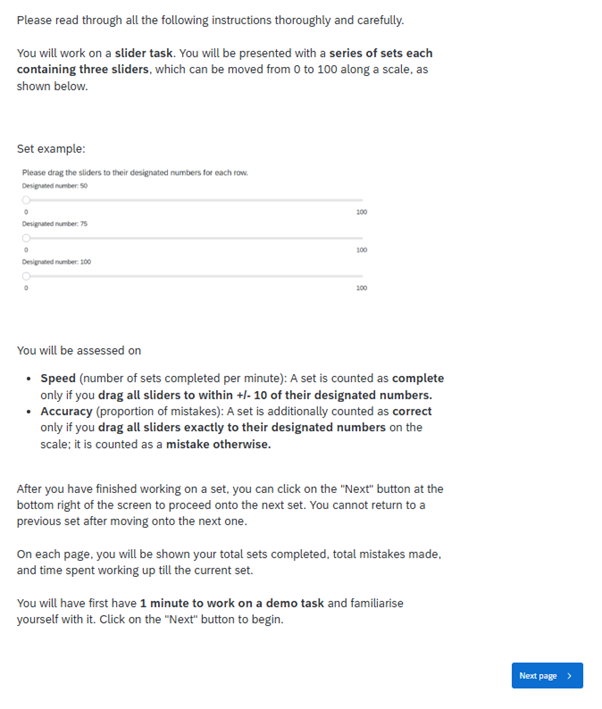
\includegraphics[keepaspectratio]{survey-screenshots/common-instructions.png}}

}

\caption{\label{fig-common-instructions}Common instructions for all
subjects}

\end{figure}%

\begin{figure}

\centering{

\pandocbounded{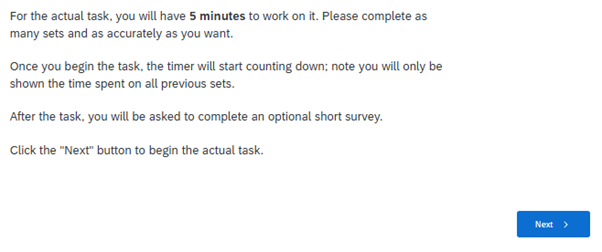
\includegraphics[keepaspectratio]{survey-screenshots/treatment1-instructions.png}}

}

\caption{\label{fig-treatment1-instructions}Treatment 1 instructions}

\end{figure}%

\begin{figure}

\centering{

\pandocbounded{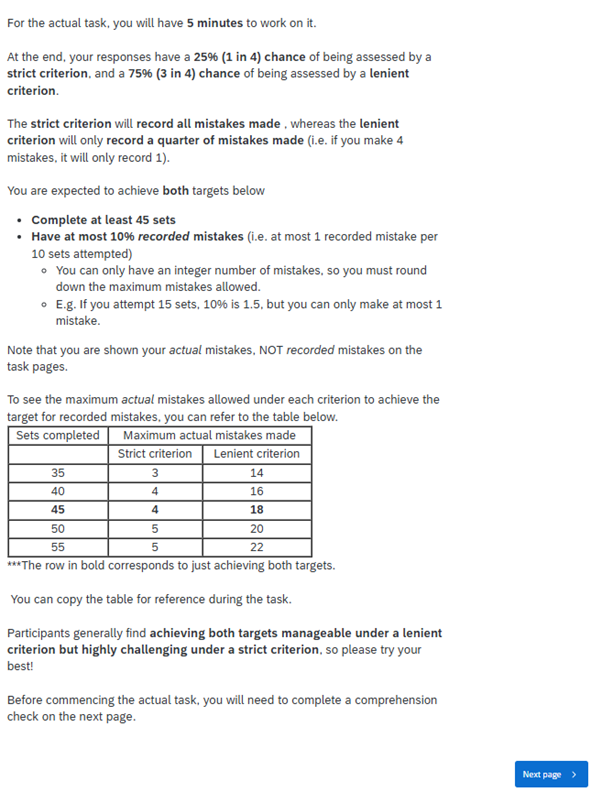
\includegraphics[keepaspectratio]{survey-screenshots/treatment2-instructions.png}}

}

\caption{\label{fig-treatment2-instructions}Treatment 2 instructions}

\end{figure}%

\begin{figure}

\centering{

\pandocbounded{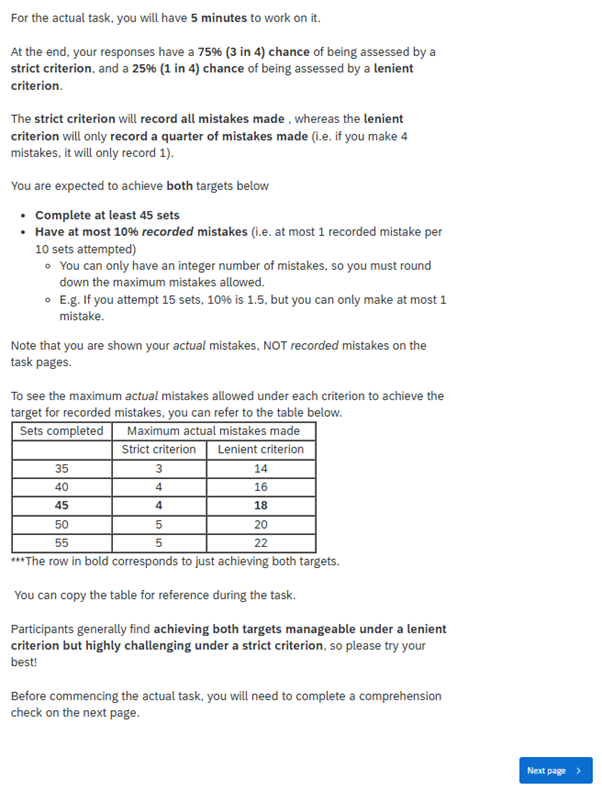
\includegraphics[keepaspectratio]{survey-screenshots/treatment3-instructions.png}}

}

\caption{\label{fig-treatment3-instructions}Treatment 3 instructions}

\end{figure}%

\begin{figure}

\centering{

\pandocbounded{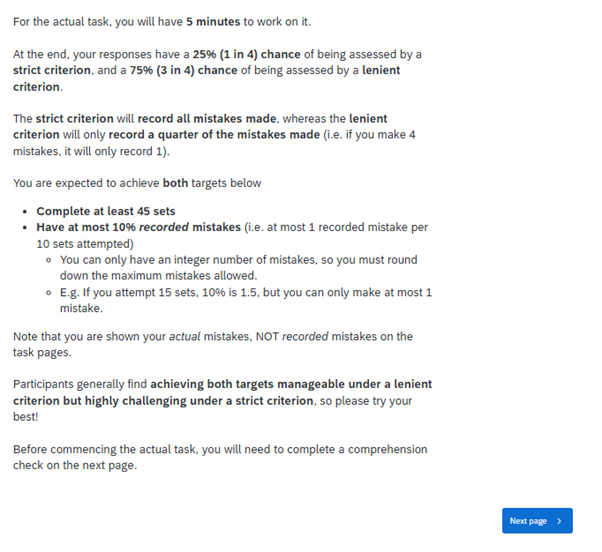
\includegraphics[keepaspectratio]{survey-screenshots/treatment4-instructions.png}}

}

\caption{\label{fig-treatment4-instructions}Treatment 4 instructions}

\end{figure}%

\begin{figure}

\centering{

\pandocbounded{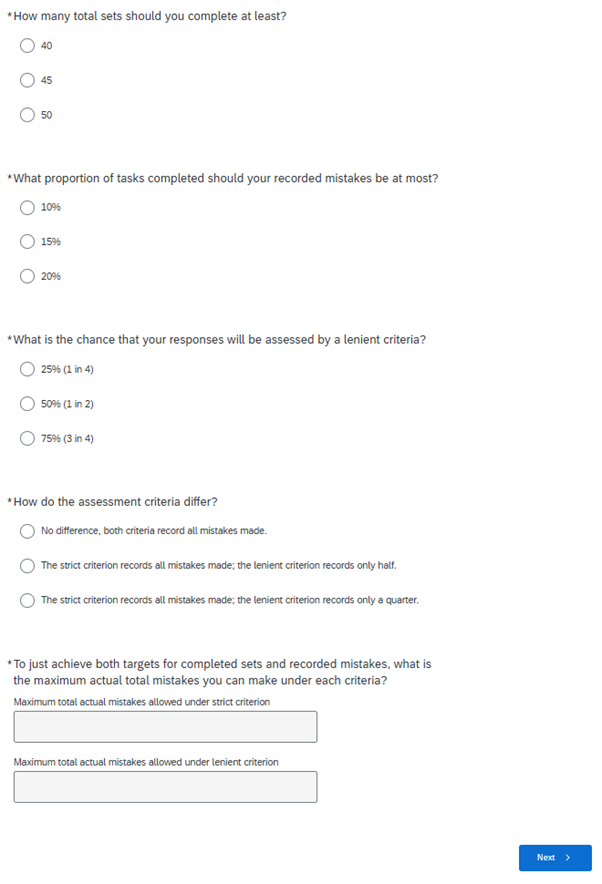
\includegraphics[keepaspectratio]{survey-screenshots/comprehension-check.png}}

}

\caption{\label{fig-compre-check}Comprehension check: last question only
for treatments 2 and 3}

\end{figure}%

\begin{figure}

\centering{

\pandocbounded{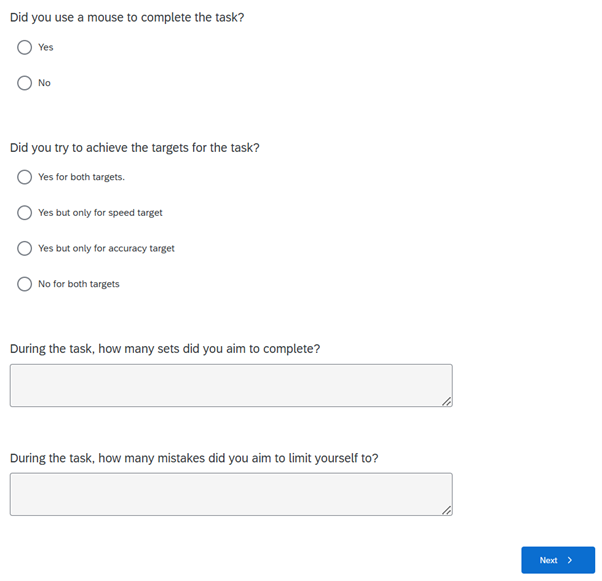
\includegraphics[keepaspectratio]{survey-screenshots/task-reflection-1.png}}

}

\caption{\label{fig-task-reflection-1}Task reflection page 1}

\end{figure}%

\begin{figure}

\centering{

\pandocbounded{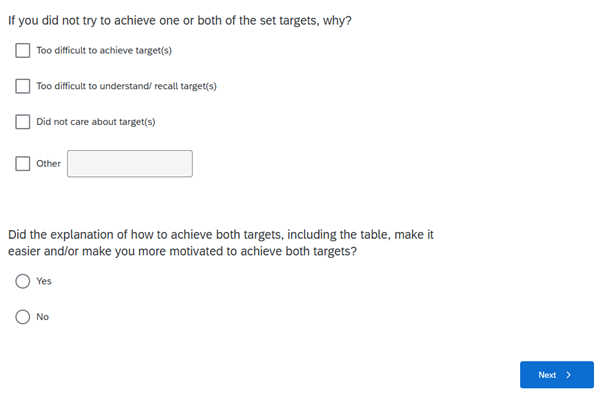
\includegraphics[keepaspectratio]{survey-screenshots/task-reflection-2.png}}

}

\caption{\label{fig-task-reflection-2}Task reflection page 2}

\end{figure}%

\begin{figure}

\centering{

\pandocbounded{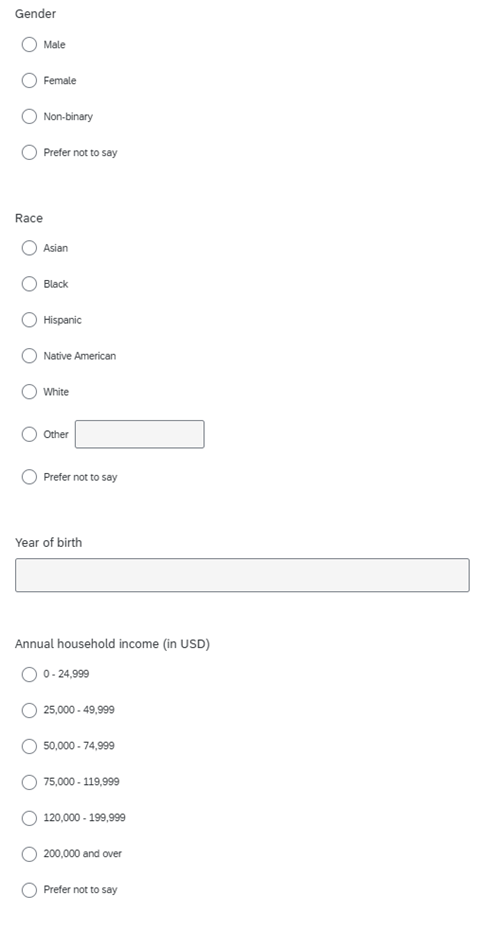
\includegraphics[keepaspectratio]{survey-screenshots/demographic-survey-1.png}}

}

\caption{\label{fig-demographic-survey-1}Demographic survey page 1}

\end{figure}%

\begin{figure}

\centering{

\pandocbounded{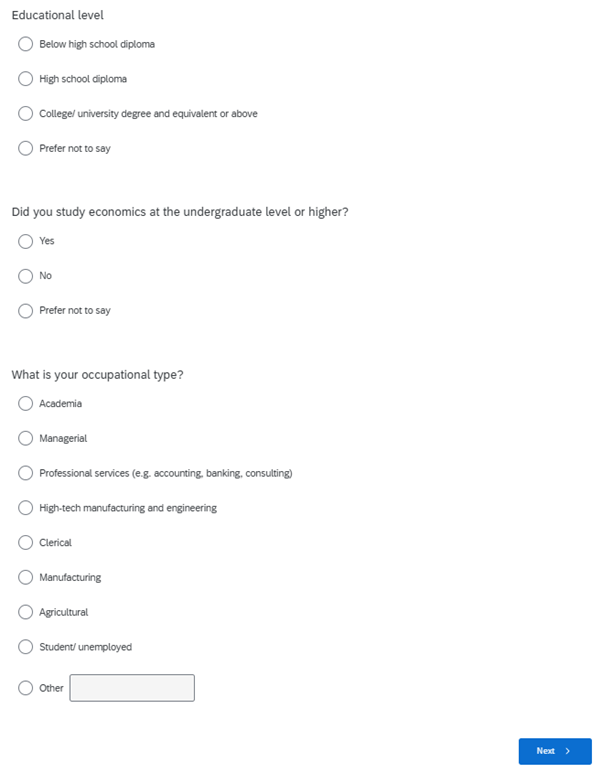
\includegraphics[keepaspectratio]{survey-screenshots/demographic-survey-2.png}}

}

\caption{\label{fig-demographic-survey-2}Demographic survey page 2}

\end{figure}%

\begin{figure}

\centering{

\pandocbounded{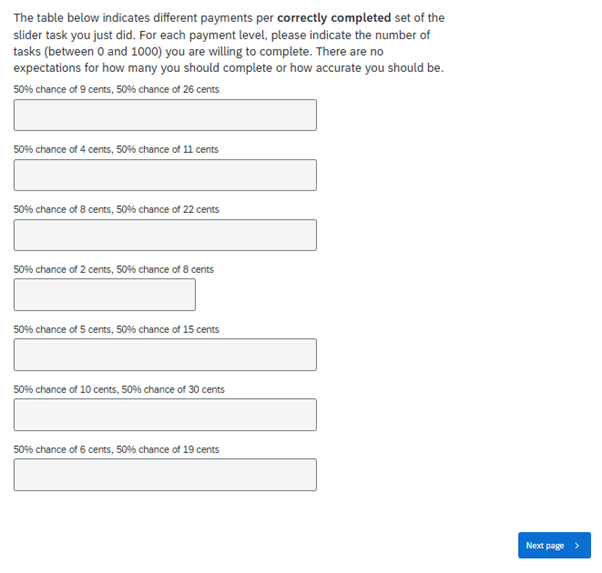
\includegraphics[keepaspectratio]{survey-screenshots/loss-aversion-survey-1.png}}

}

\caption{\label{fig-loss-aversion-survey-1}Loss aversion survey page 1:
pages and payment structures presented in random order}

\end{figure}%

\begin{figure}

\centering{

\pandocbounded{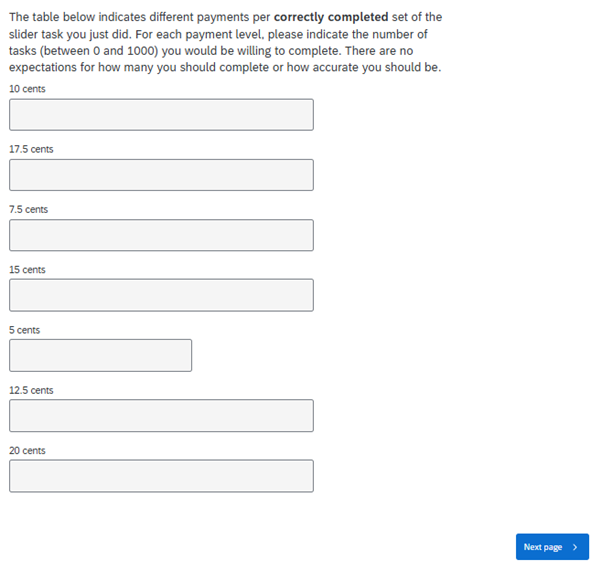
\includegraphics[keepaspectratio]{survey-screenshots/loss-aversion-survey-2.png}}

}

\caption{\label{fig-loss-aversion-survey-2}Loss aversion survey page 2:
pages and payment structures presented in random order}

\end{figure}%




\end{document}
